\section{Detekcja}

\begin{longtable}{|c|c|c|c|c|c|} 
\hline
  		& \bfseries Wejście & \bfseries Haar & \bfseries Dnn & \bfseries Azure \\
  		\hline
  		1&		\begin{minipage}{.2\textwidth}
      	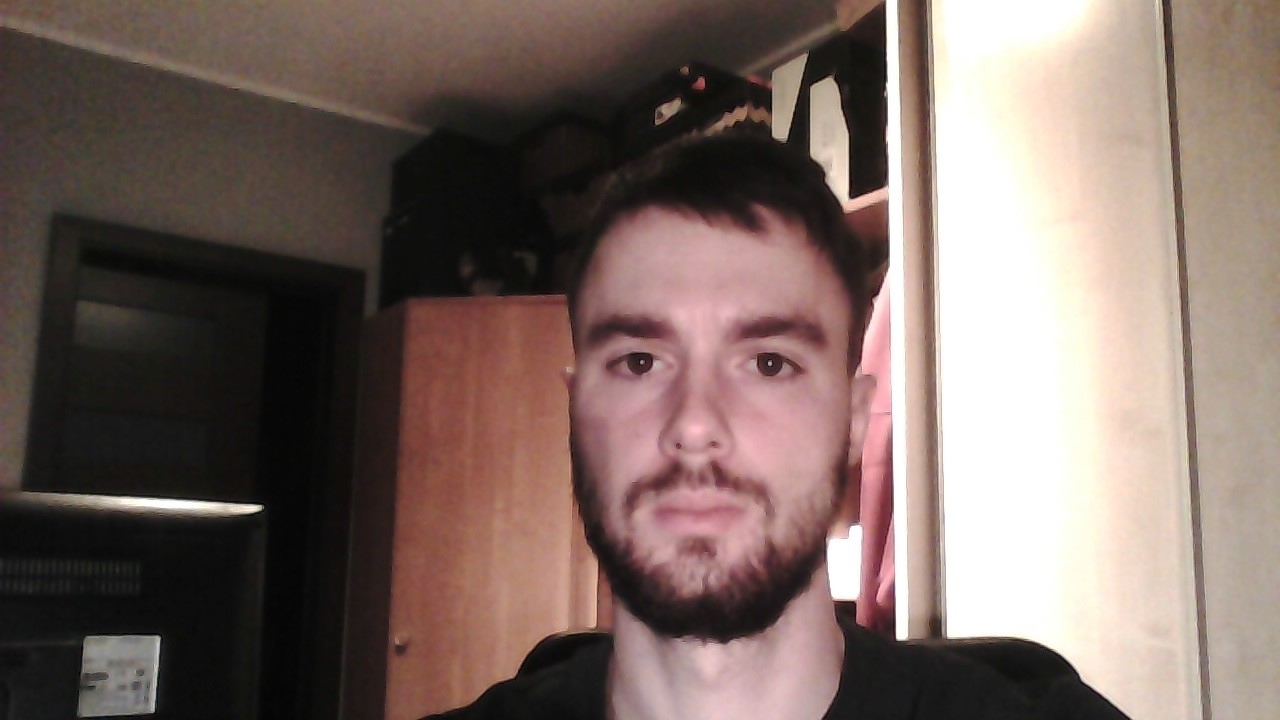
\includegraphics[width=\linewidth, height=20mm]{detekcja/3_input.jpg}
    	\end{minipage}
		& 
		\begin{minipage}{.2\textwidth}
      	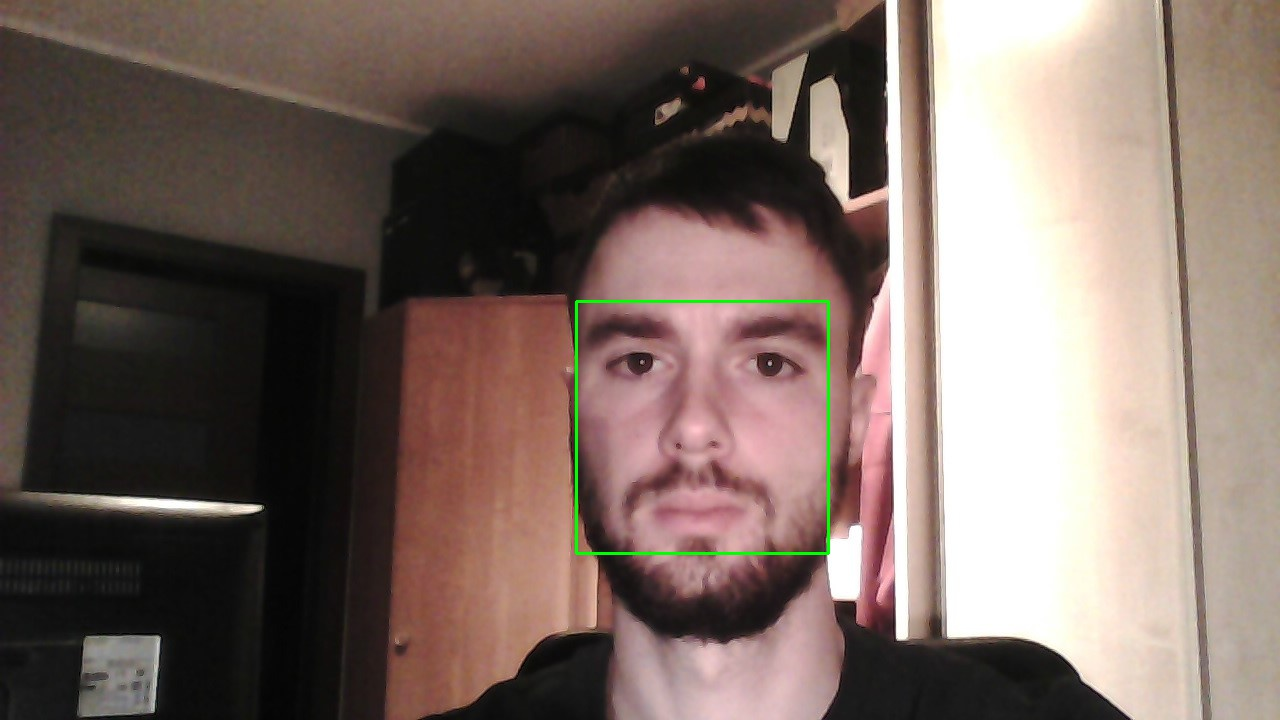
\includegraphics[width=\linewidth, height=20mm]{detekcja/3_haar.jpg}
    	\end{minipage}
		& 
		\begin{minipage}{.2\textwidth}
      	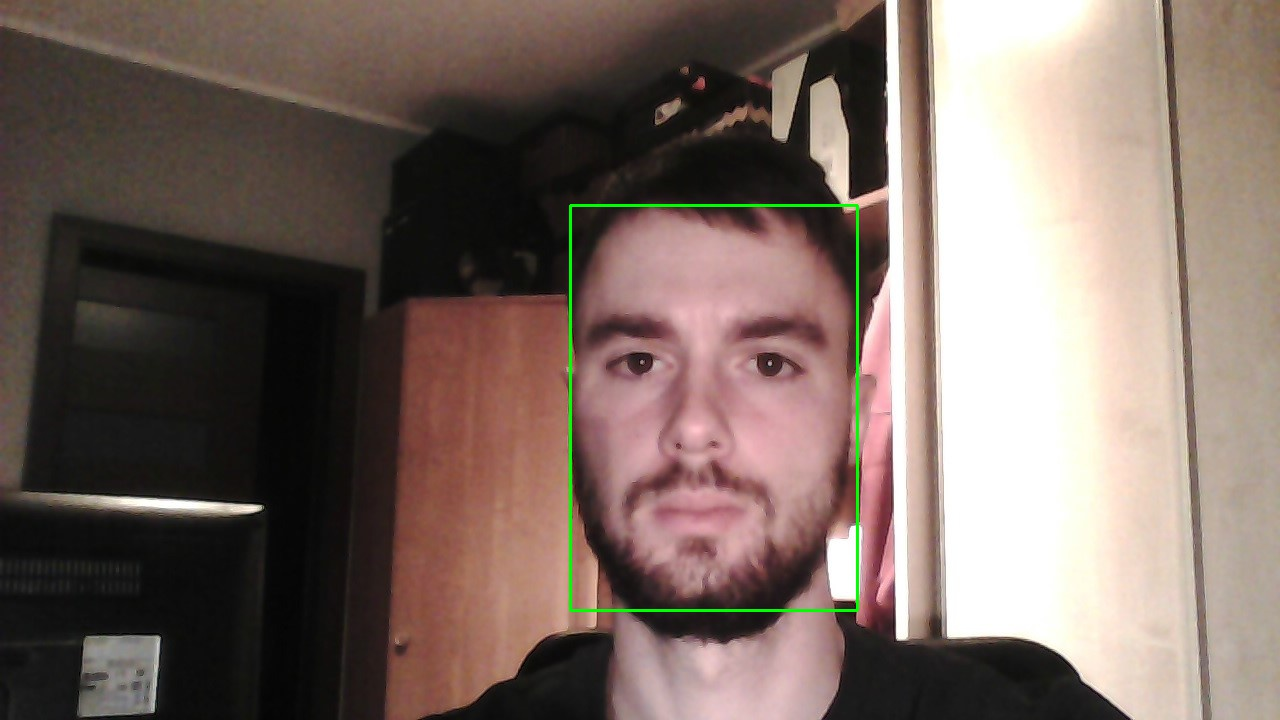
\includegraphics[width=\linewidth, height=20mm]{detekcja/3_dnn.jpg}
    	\end{minipage}
		& 
		\begin{minipage}{.2\textwidth}
      	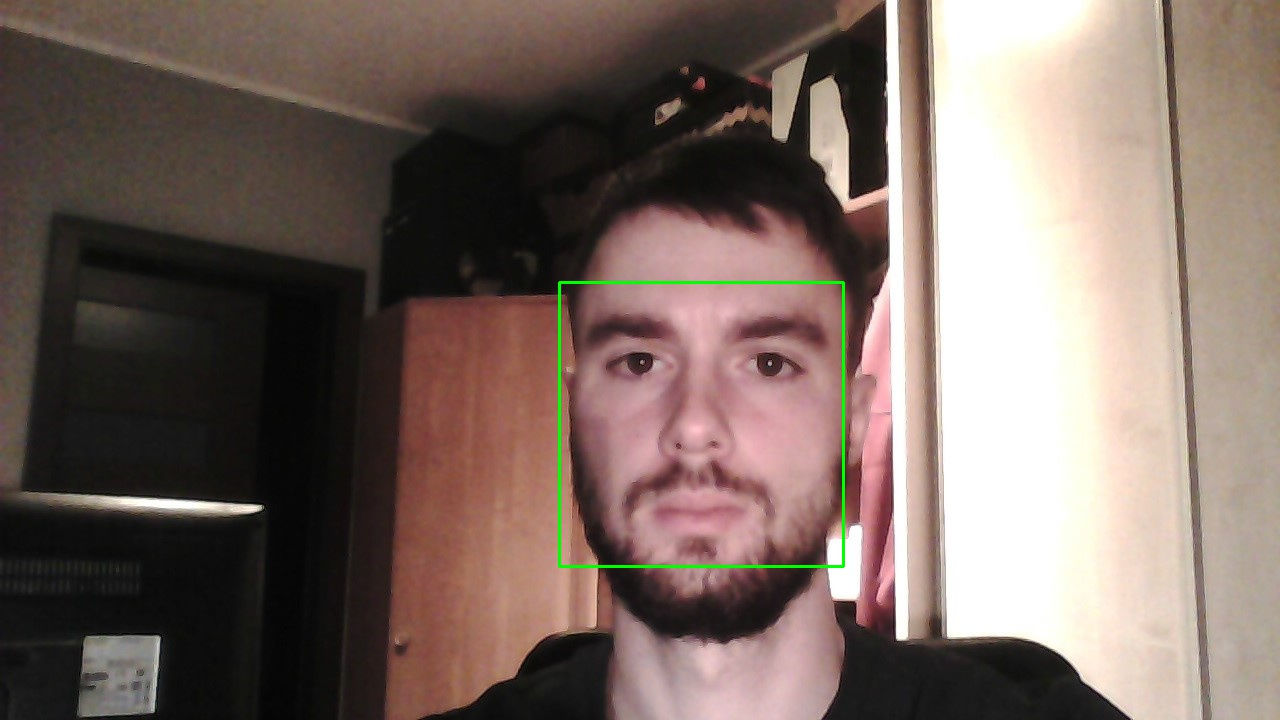
\includegraphics[width=\linewidth, height=20mm]{detekcja/3_azure.jpg}
    	\end{minipage}	
		\\
  		\hline
  		2&		\begin{minipage}{.2\textwidth}
      	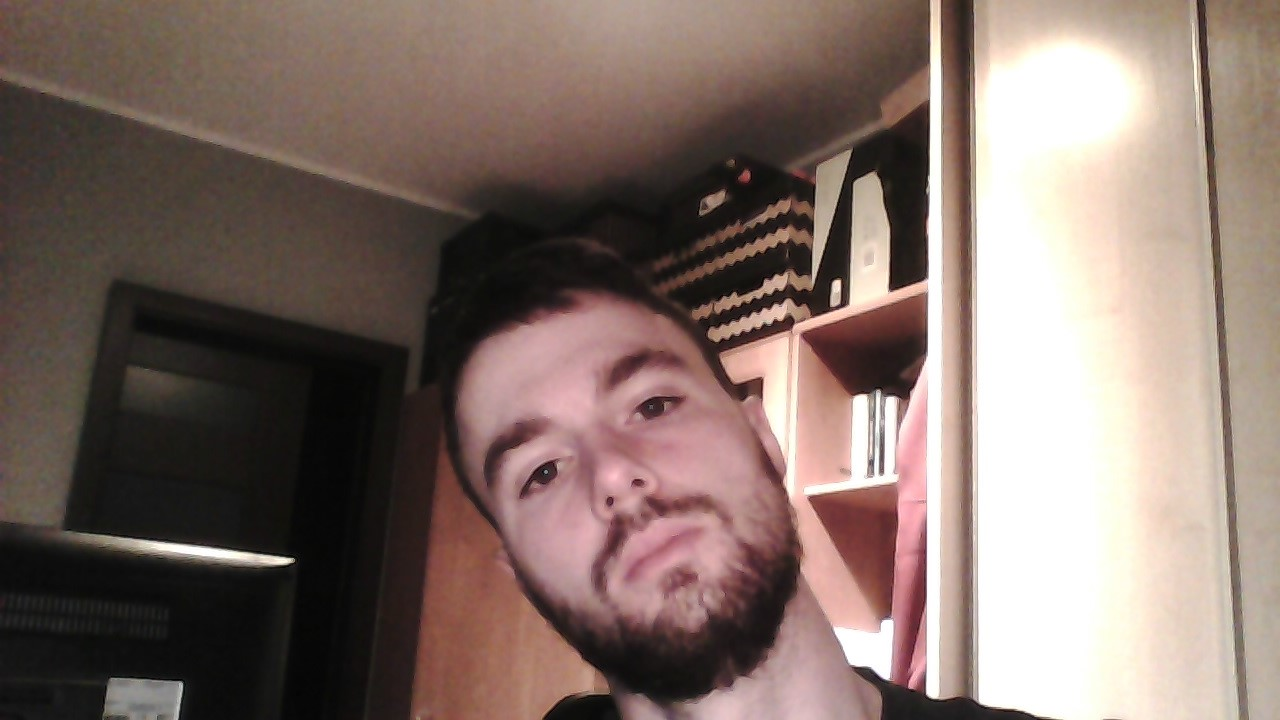
\includegraphics[width=\linewidth, height=20mm]{detekcja/4_input.jpg}
    	\end{minipage}
		& 
		\begin{minipage}{.2\textwidth}
      	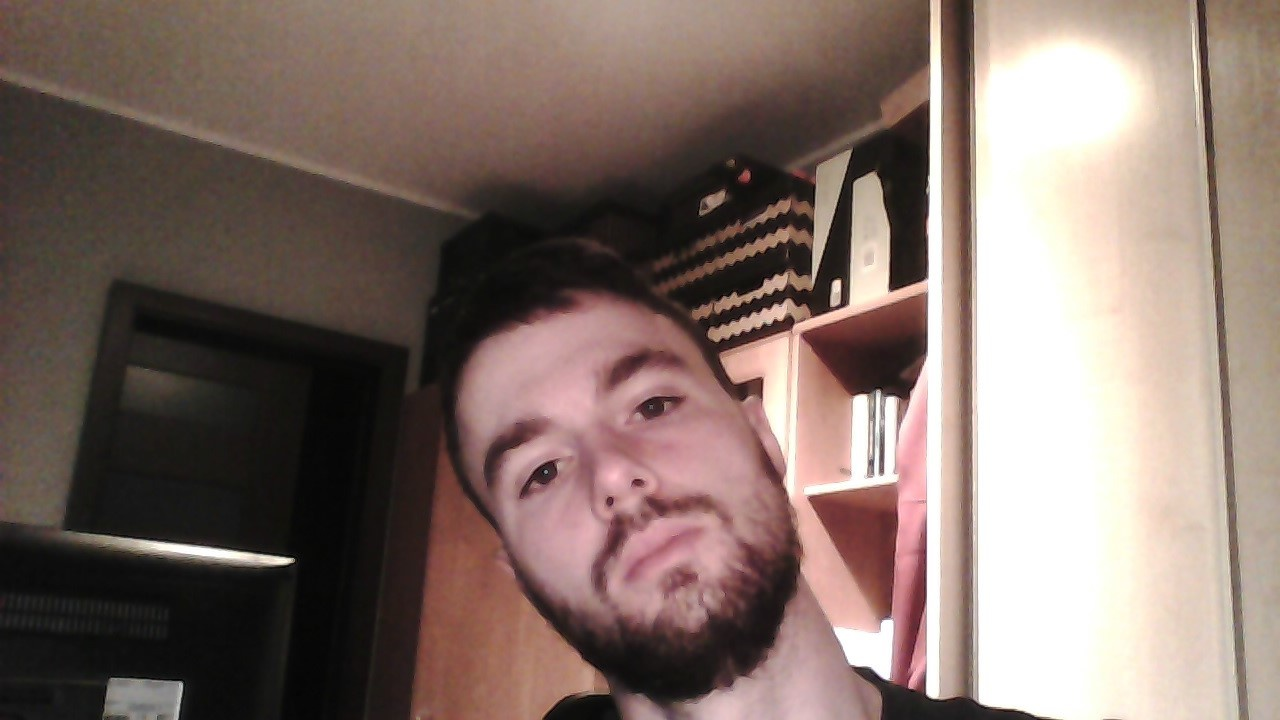
\includegraphics[width=\linewidth, height=20mm]{detekcja/4_haar.jpg}
    	\end{minipage}
		& 
		\begin{minipage}{.2\textwidth}
      	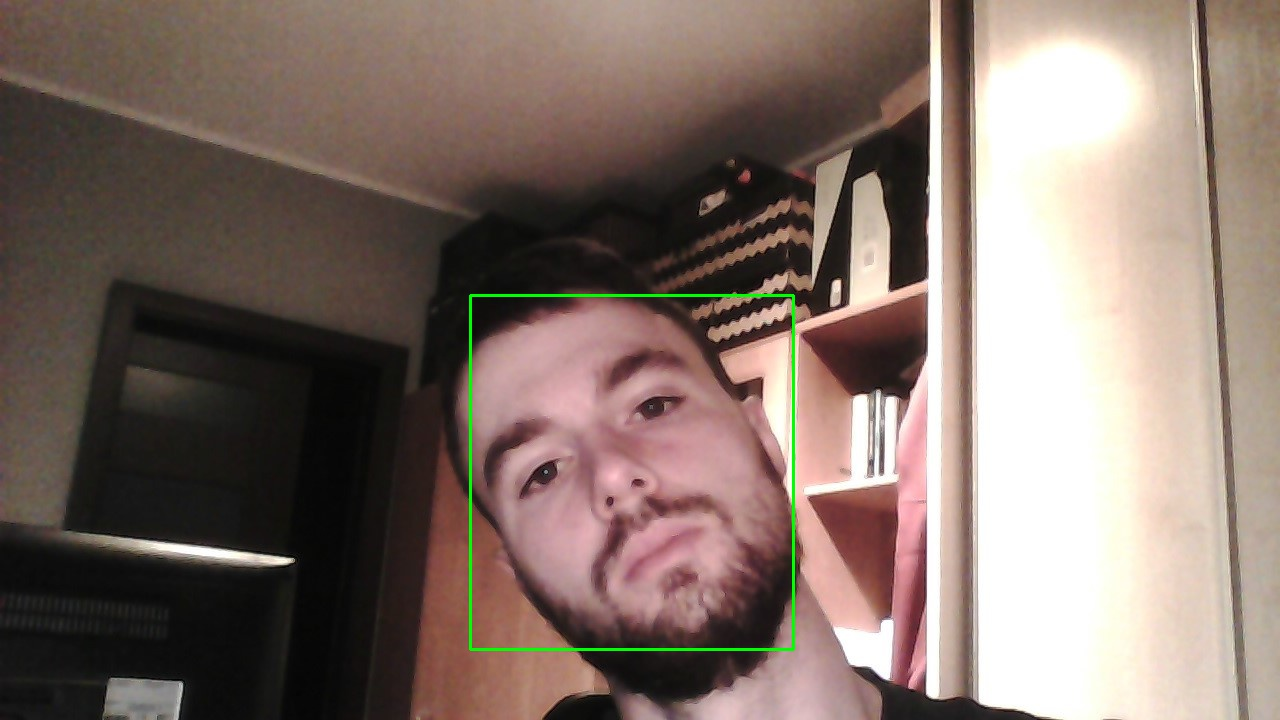
\includegraphics[width=\linewidth, height=20mm]{detekcja/4_dnn.jpg}
    	\end{minipage}
		& 
		\begin{minipage}{.2\textwidth}
      	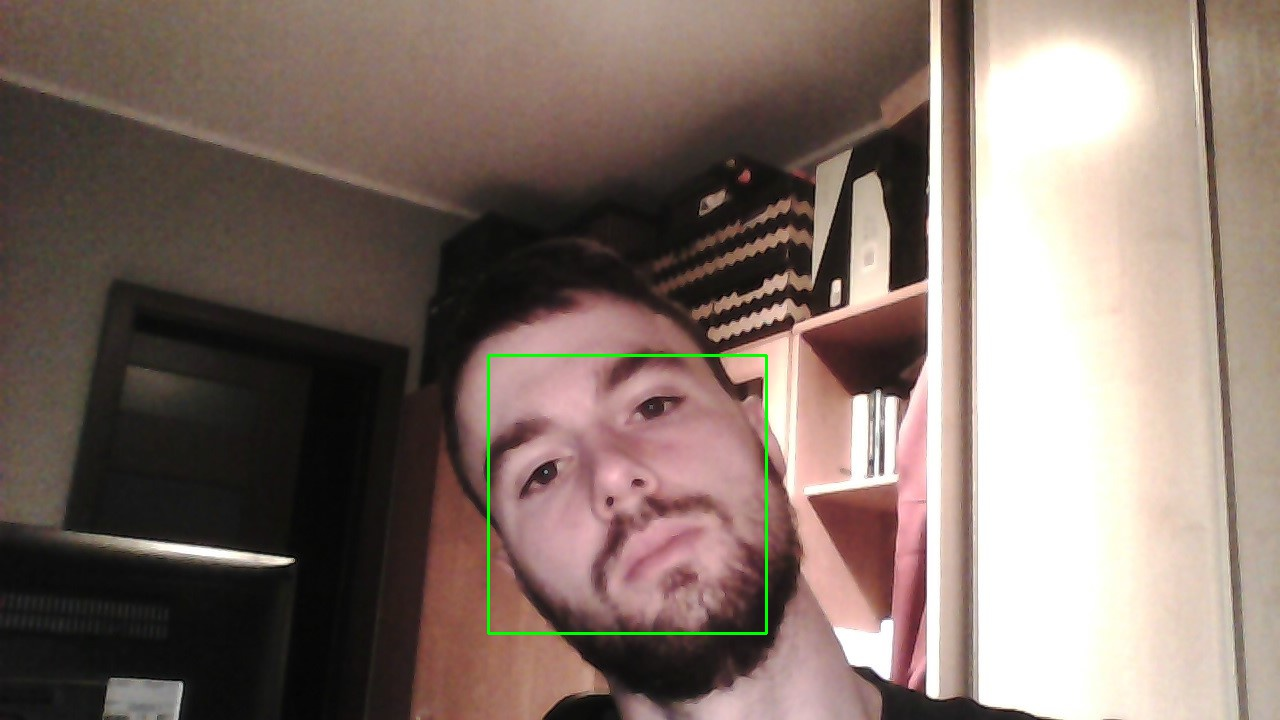
\includegraphics[width=\linewidth, height=20mm]{detekcja/4_azure.jpg}
    	\end{minipage}	
		\\
  		\hline
  		3& 		\begin{minipage}{.2\textwidth}
      	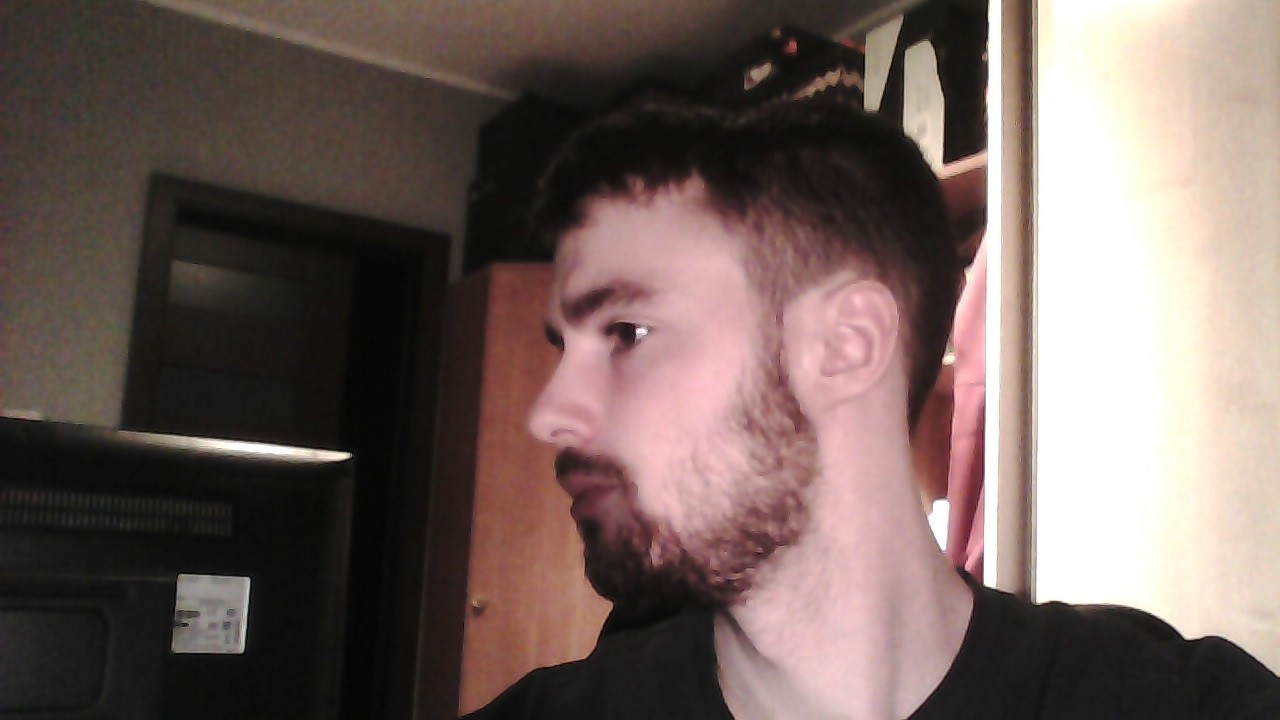
\includegraphics[width=\linewidth, height=20mm]{detekcja/5_input.jpg}
    	\end{minipage}
		& 
		\begin{minipage}{.2\textwidth}
      	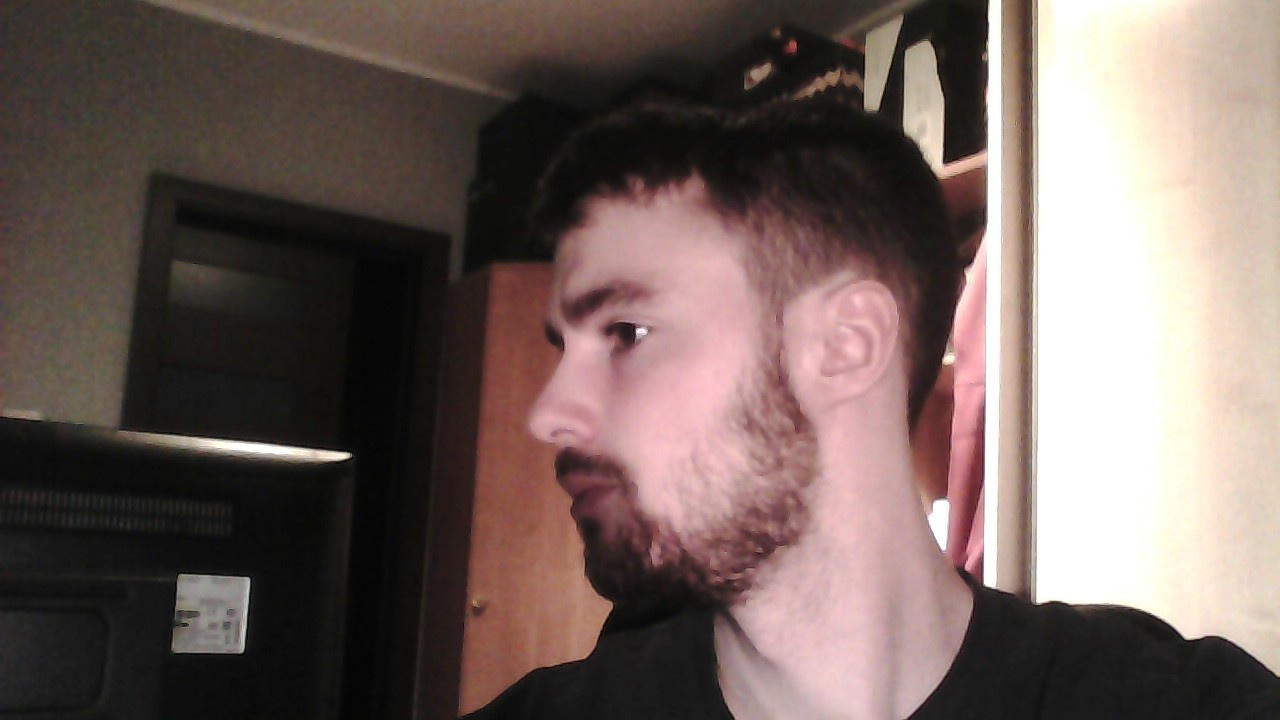
\includegraphics[width=\linewidth, height=20mm]{detekcja/5_haar.jpg}
    	\end{minipage}
		& 
		\begin{minipage}{.2\textwidth}
      	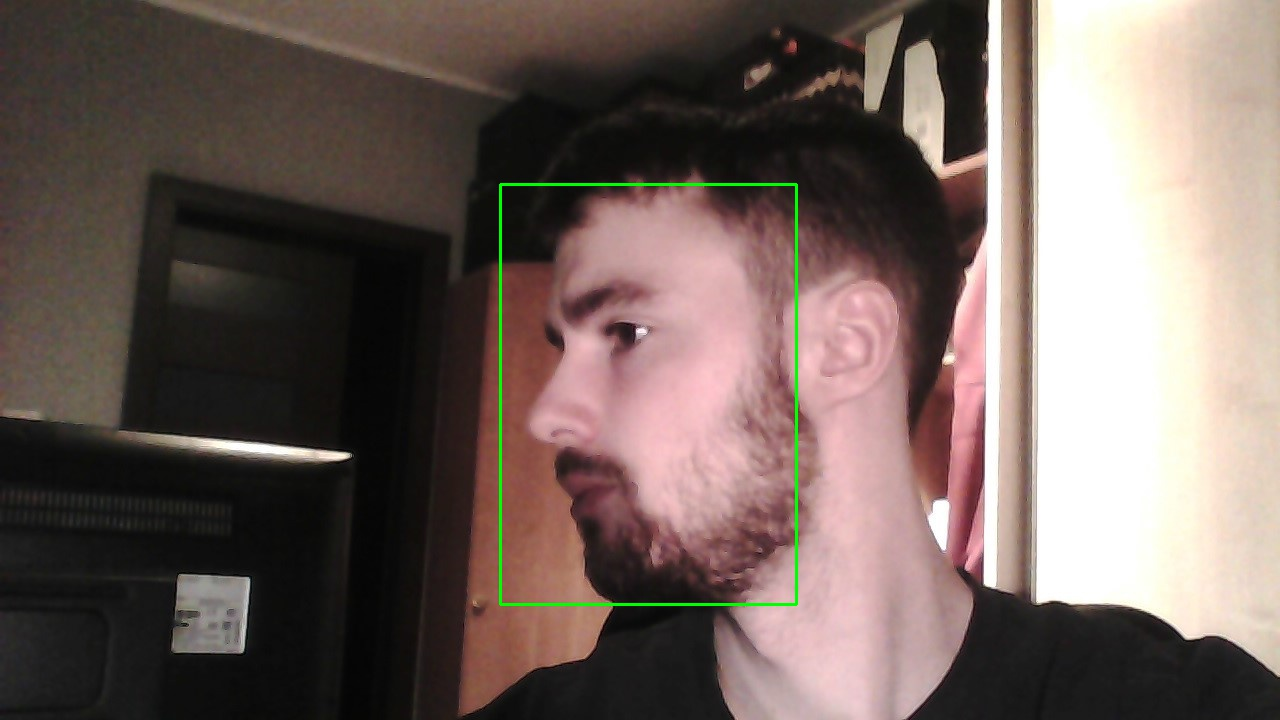
\includegraphics[width=\linewidth, height=20mm]{detekcja/5_dnn.jpg}
    	\end{minipage}
		& 
		\begin{minipage}{.2\textwidth}
      	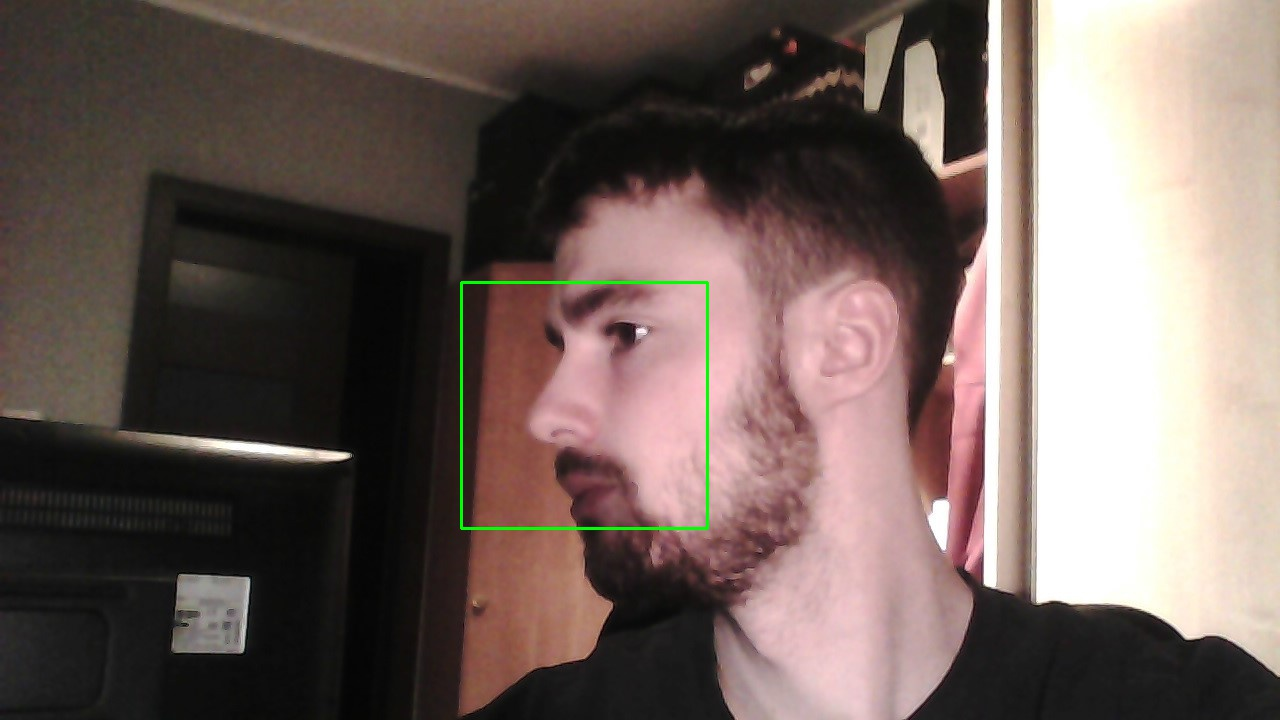
\includegraphics[width=\linewidth, height=20mm]{detekcja/5_azure.jpg}
    	\end{minipage}	
		\\
  		\hline
  		4&  		\begin{minipage}{.2\textwidth}
      	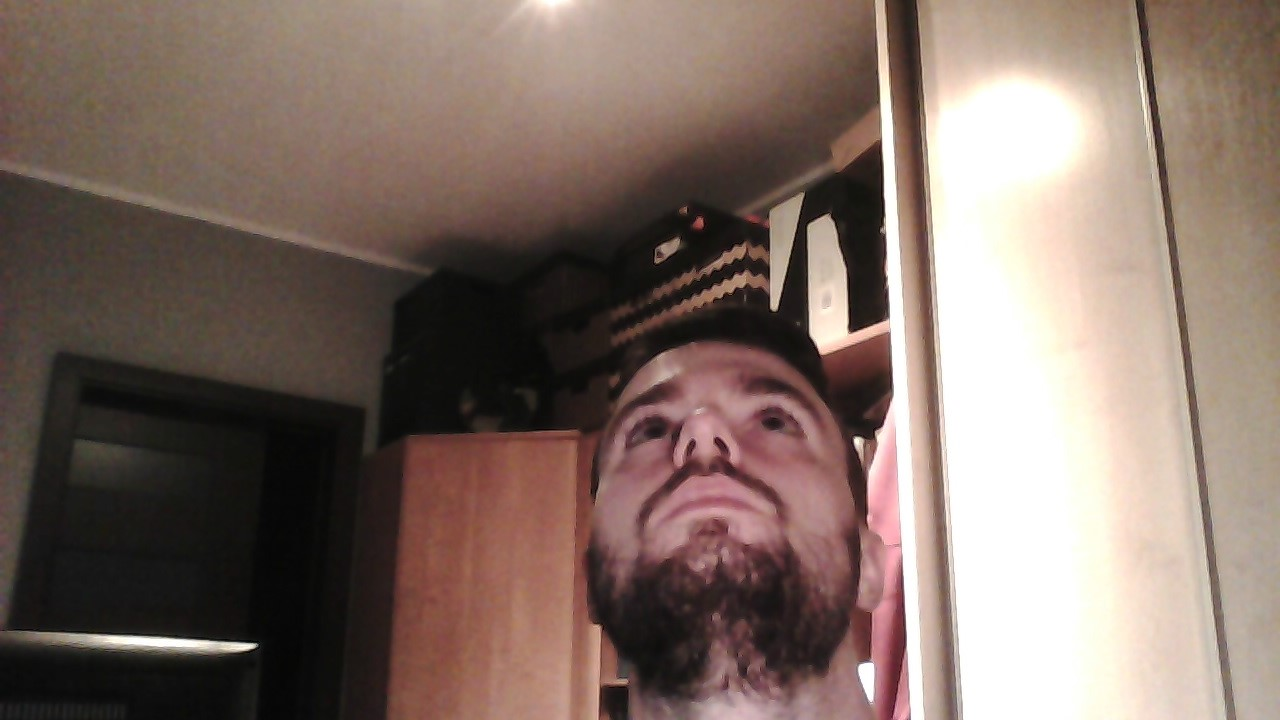
\includegraphics[width=\linewidth, height=20mm]{detekcja/6_input.jpg}
    	\end{minipage}
		& 
		\begin{minipage}{.2\textwidth}
      	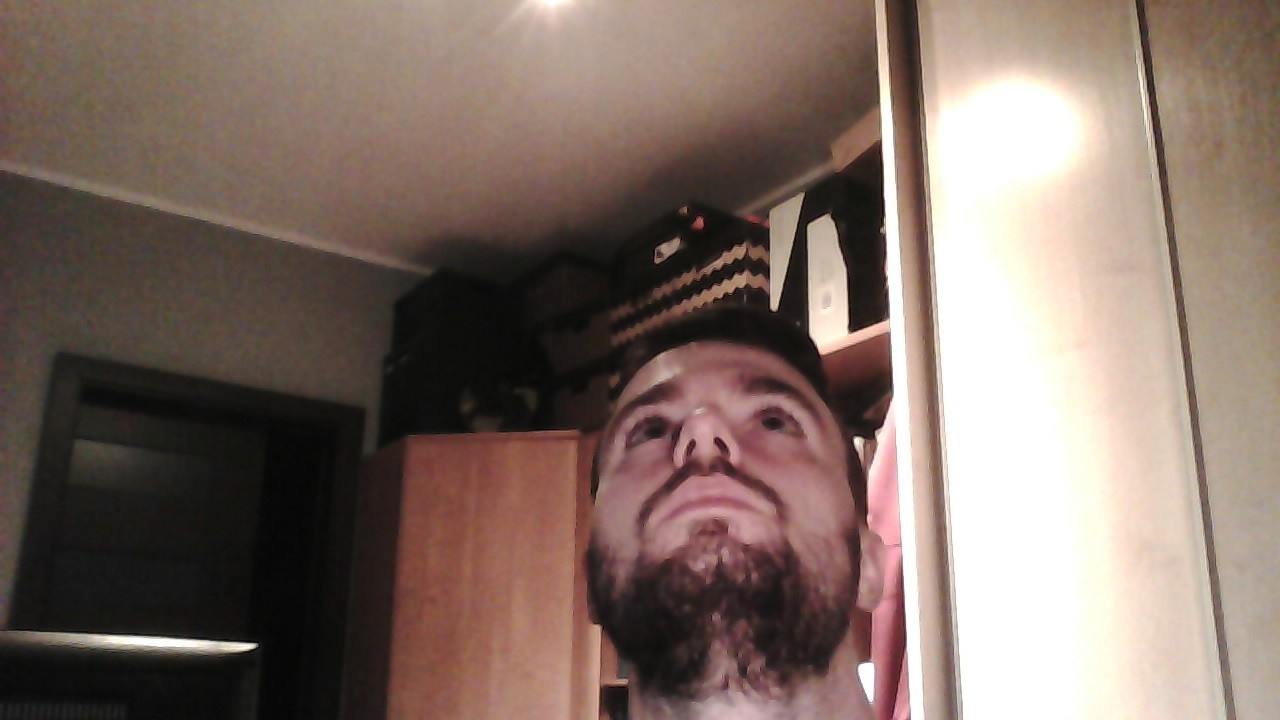
\includegraphics[width=\linewidth, height=20mm]{detekcja/6_haar.jpg}
    	\end{minipage}
		& 
		\begin{minipage}{.2\textwidth}
      	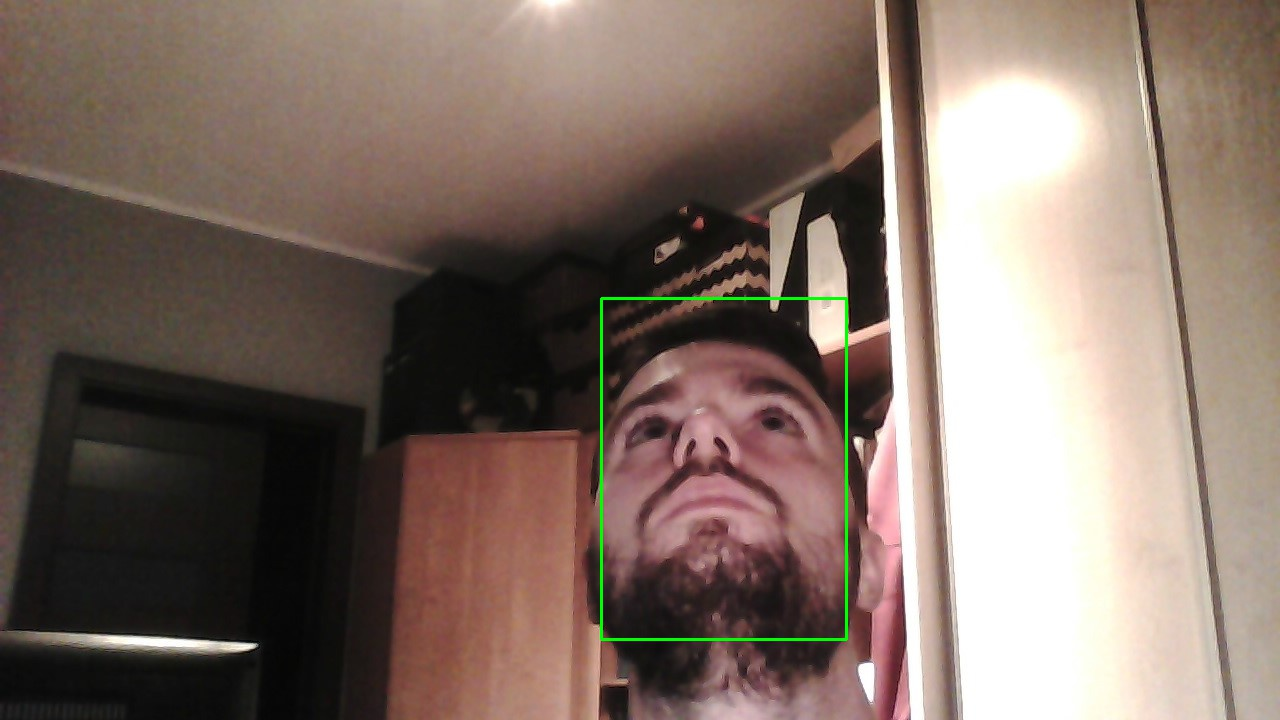
\includegraphics[width=\linewidth, height=20mm]{detekcja/6_dnn.jpg}
    	\end{minipage}
		& 
		\begin{minipage}{.2\textwidth}
      	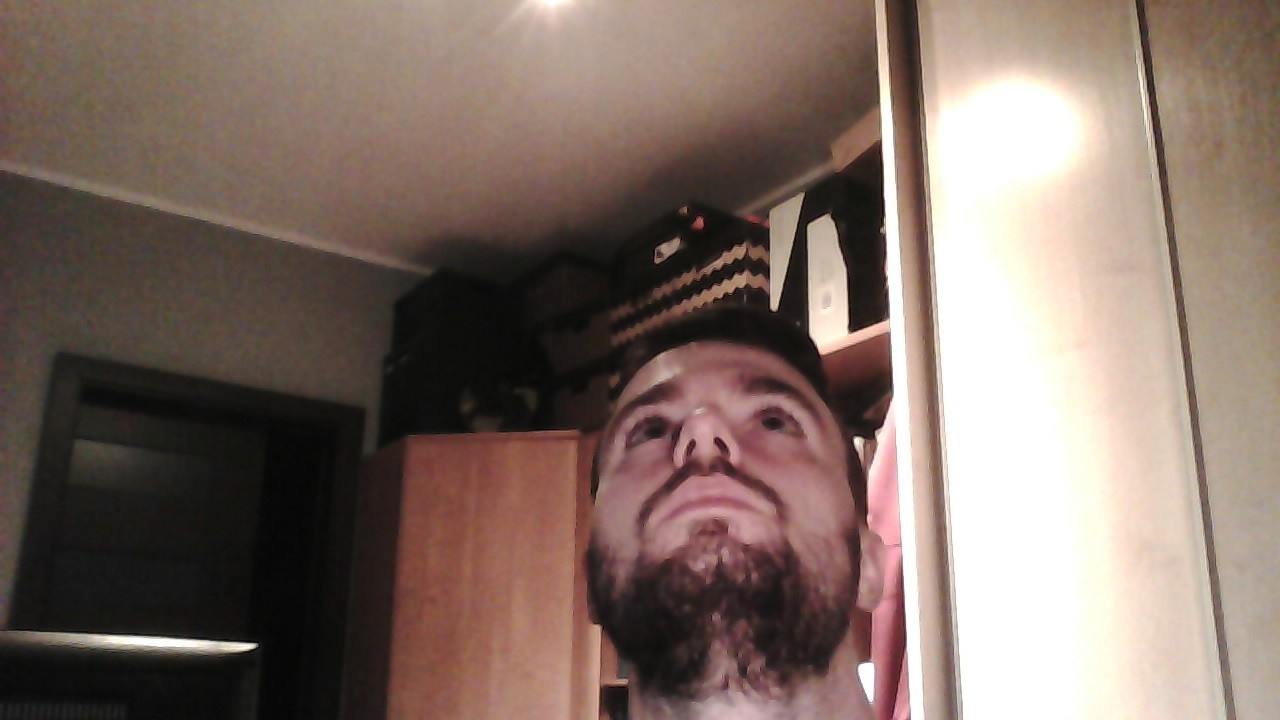
\includegraphics[width=\linewidth, height=20mm]{detekcja/6_azure.jpg}
    	\end{minipage}	
		\\
  		\hline
  		5&  		\begin{minipage}{.2\textwidth}
      	
\includegraphics[width=\linewidth, height=20mm]{detekcja/7_input.jpg}
    	\end{minipage}
		& 
		\begin{minipage}{.2\textwidth}
      	
\includegraphics[width=\linewidth, height=20mm]{detekcja/7_haar.jpg}
    	\end{minipage}
		& 
		\begin{minipage}{.2\textwidth}
      	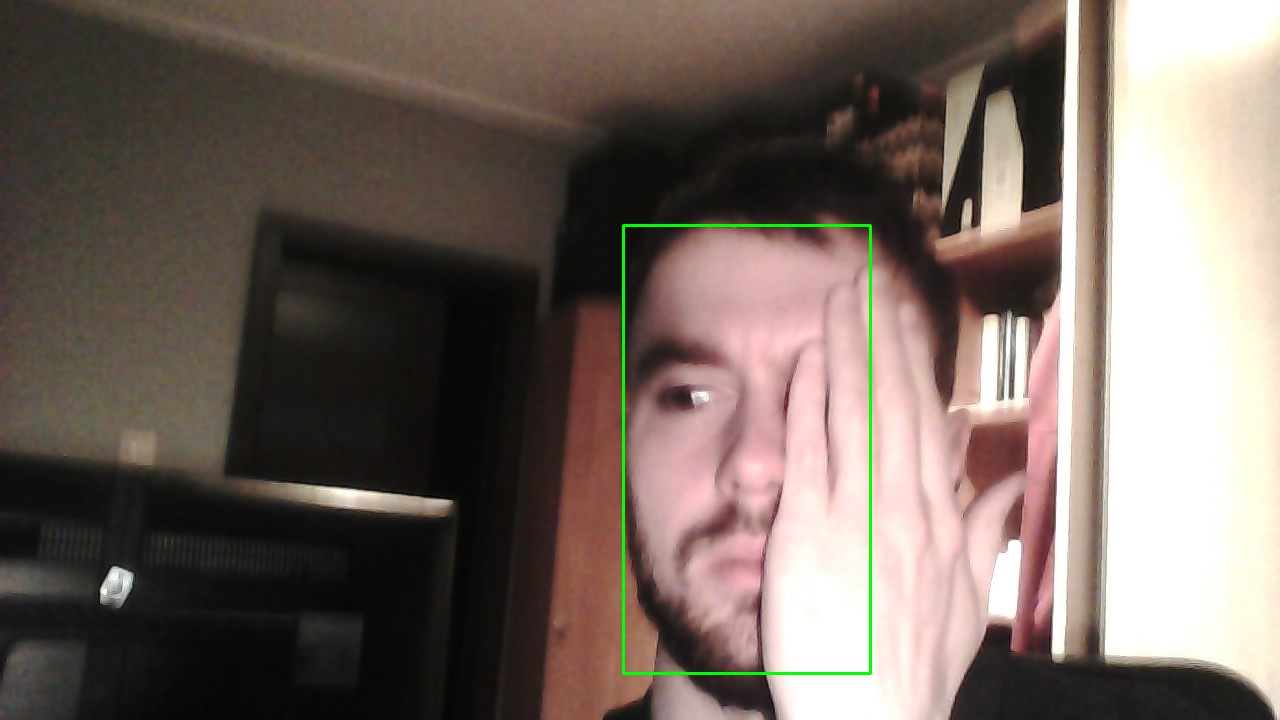
\includegraphics[width=\linewidth, height=20mm]{detekcja/7_dnn.jpg}
    	\end{minipage}
		& 
		\begin{minipage}{.2\textwidth}
      	
\includegraphics[width=\linewidth, height=20mm]{detekcja/7_azure.jpg}
    	\end{minipage}	
		\\
  		\hline
  		6&  		\begin{minipage}{.2\textwidth}
      	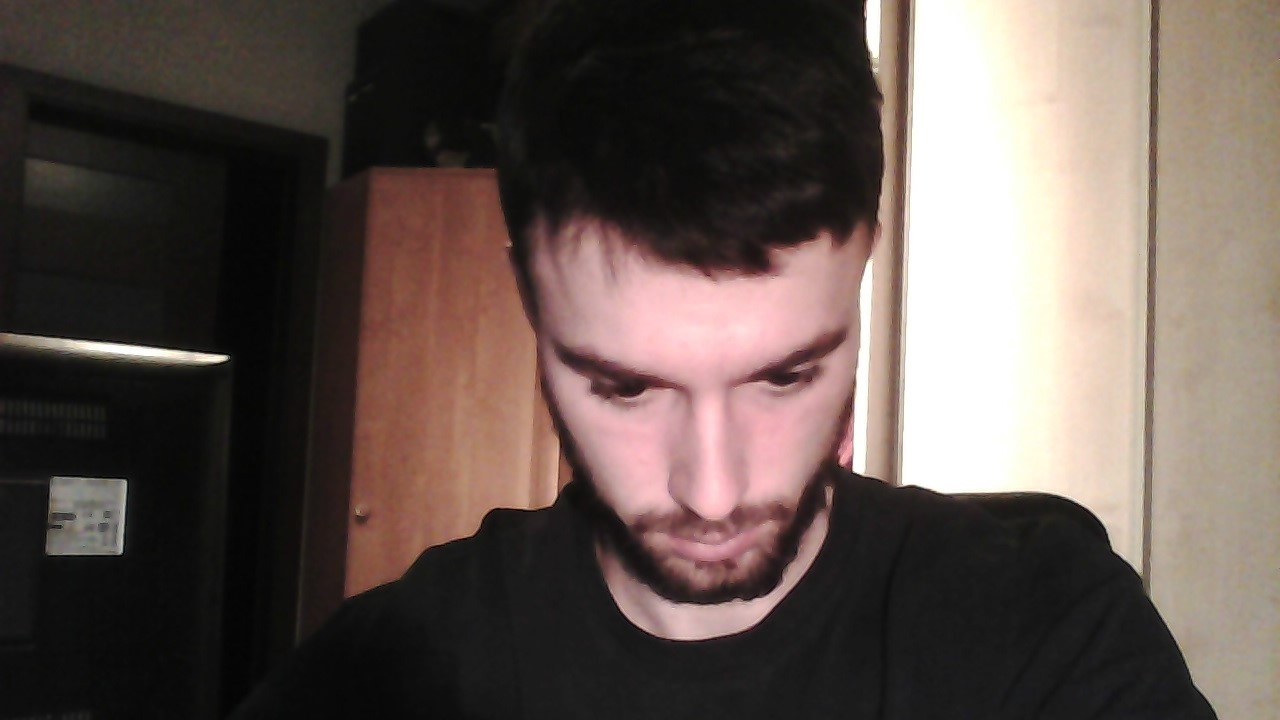
\includegraphics[width=\linewidth, height=20mm]{detekcja/8_input.jpg}
    	\end{minipage}
		& 
		\begin{minipage}{.2\textwidth}
      	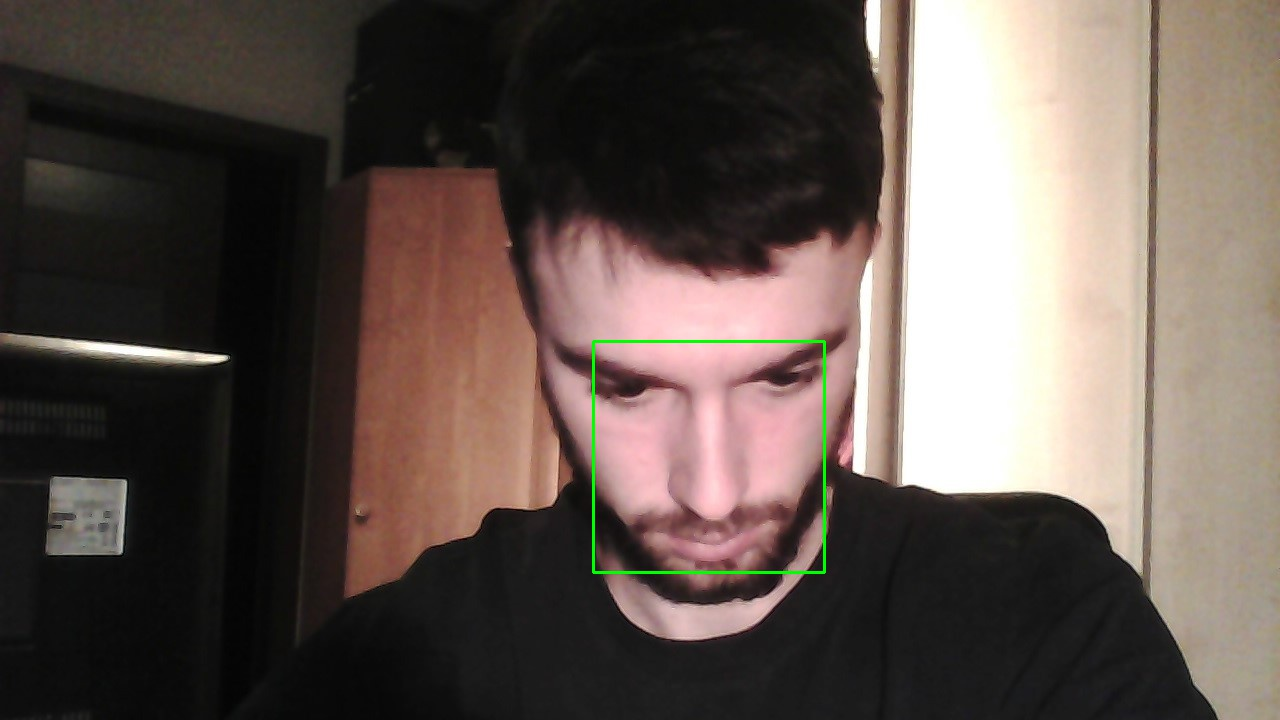
\includegraphics[width=\linewidth, height=20mm]{detekcja/8_haar.jpg}
    	\end{minipage}
		& 
		\begin{minipage}{.2\textwidth}
      	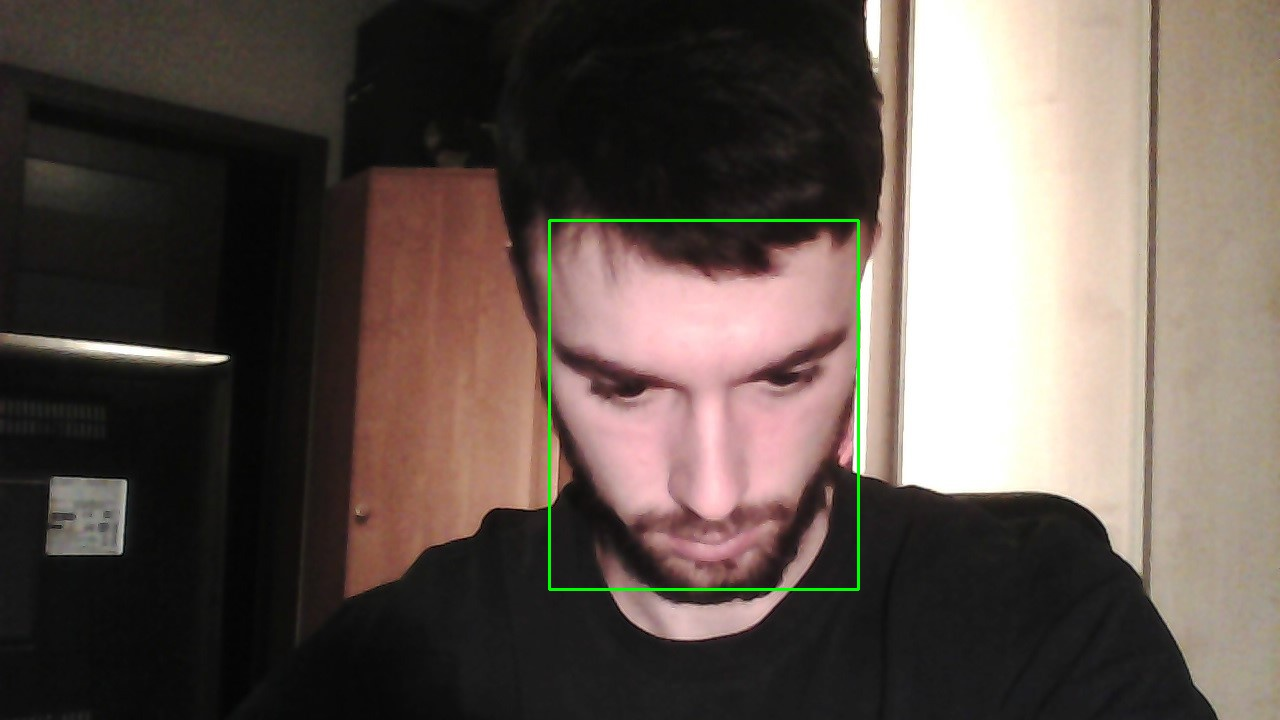
\includegraphics[width=\linewidth, height=20mm]{detekcja/8_dnn.jpg}
    	\end{minipage}
		& 
		\begin{minipage}{.2\textwidth}
      	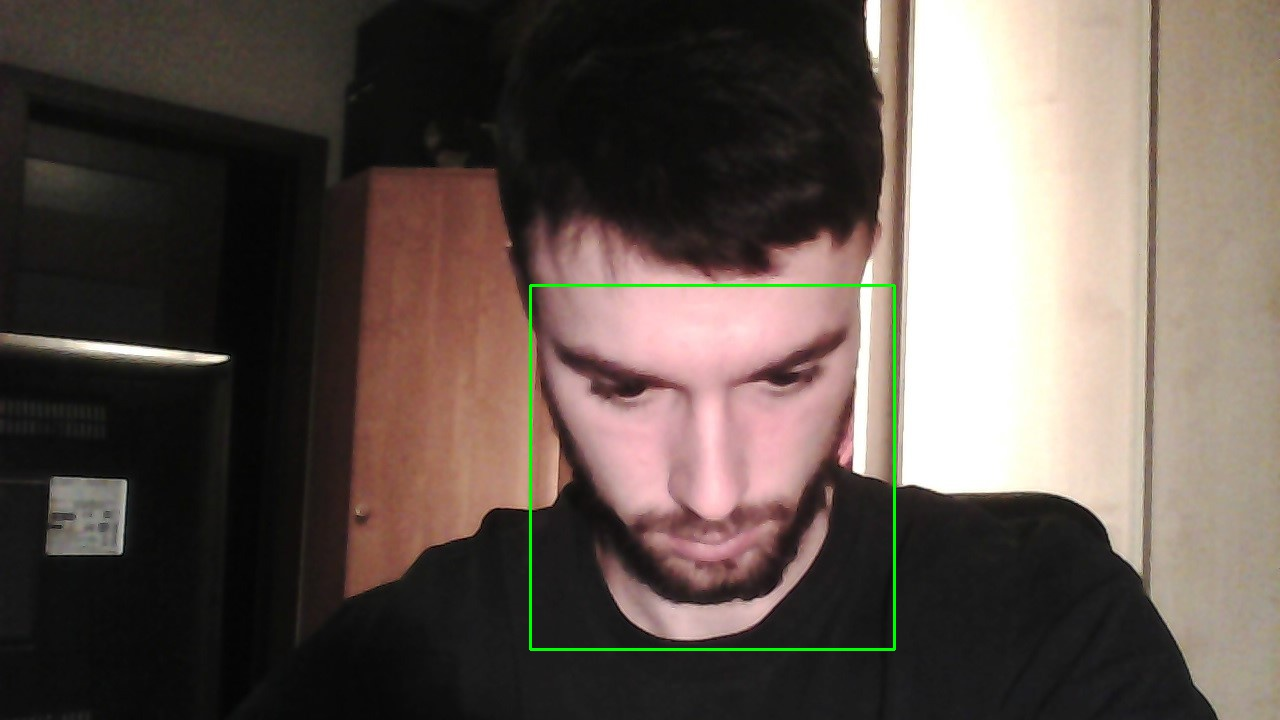
\includegraphics[width=\linewidth, height=20mm]{detekcja/8_azure.jpg}
    	\end{minipage}	
		\\
  		\hline
  		7&  		\begin{minipage}{.2\textwidth}
      	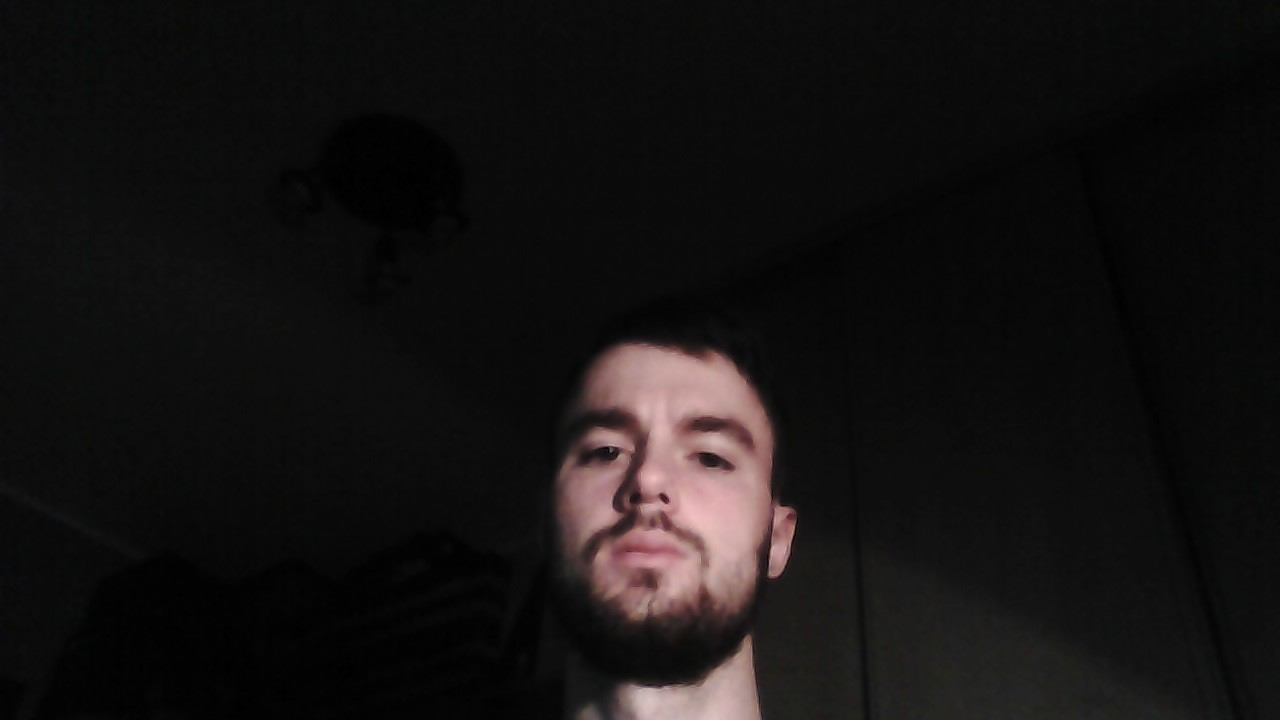
\includegraphics[width=\linewidth, height=20mm]{detekcja/9_input.jpg}
    	\end{minipage}
		& 
		\begin{minipage}{.2\textwidth}
      	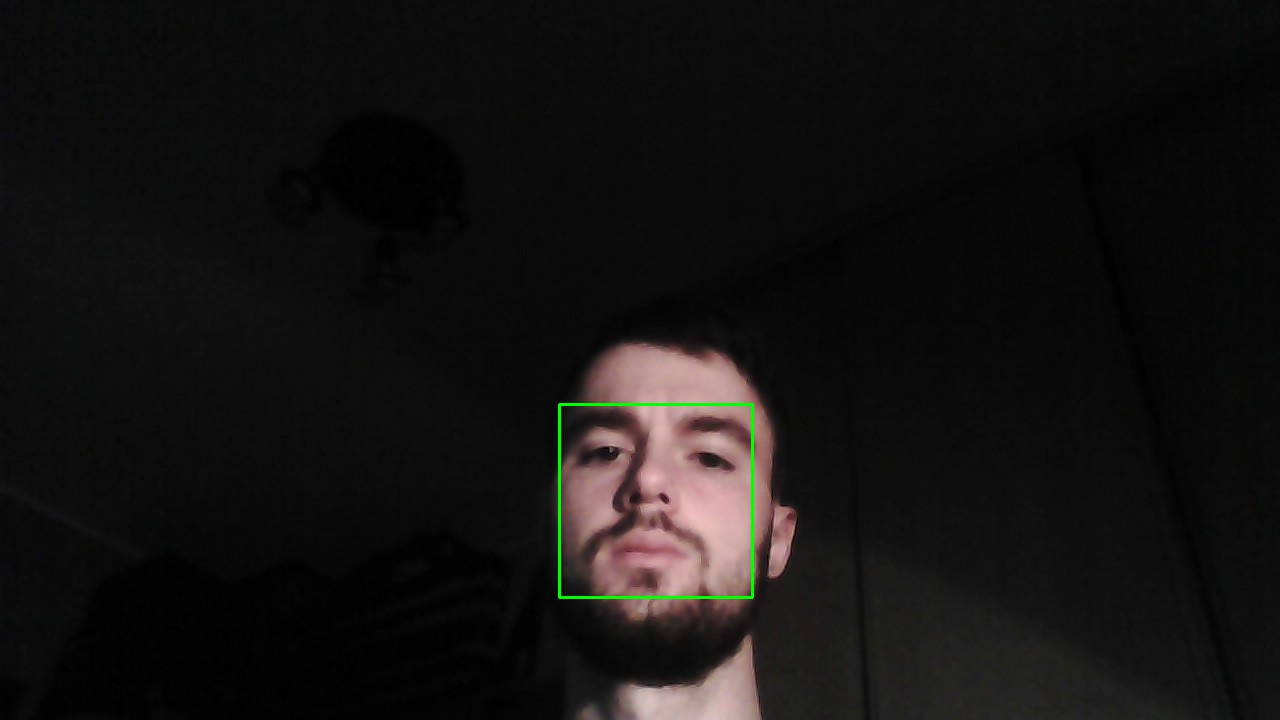
\includegraphics[width=\linewidth, height=20mm]{detekcja/9_haar.jpg}
    	\end{minipage}
		& 
		\begin{minipage}{.2\textwidth}
      	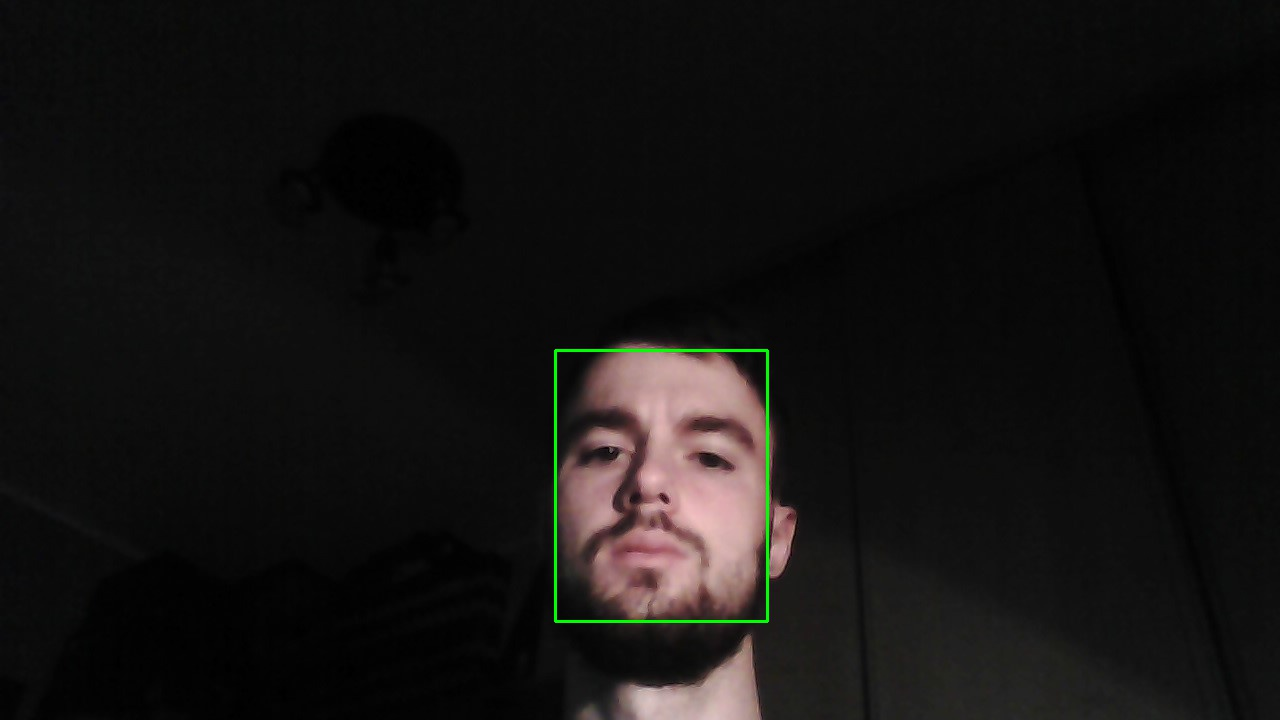
\includegraphics[width=\linewidth, height=20mm]{detekcja/9_dnn.jpg}
    	\end{minipage}
		& 
		\begin{minipage}{.2\textwidth}
      	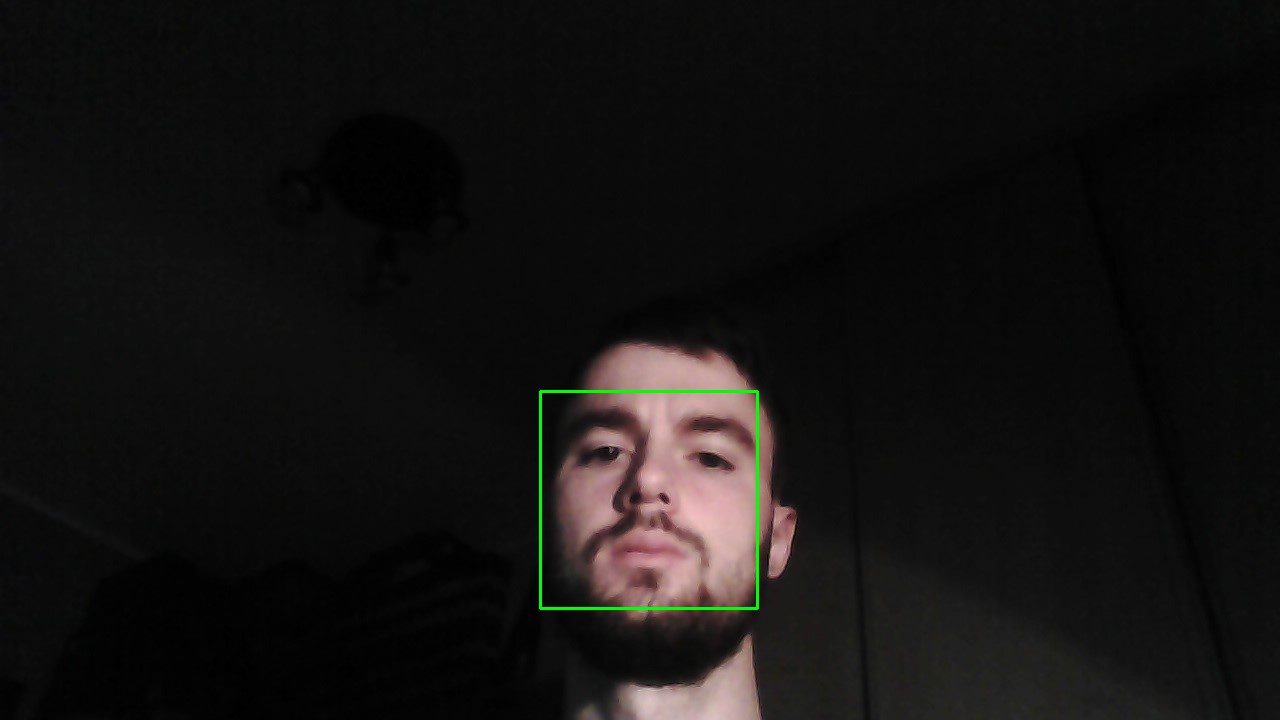
\includegraphics[width=\linewidth, height=20mm]{detekcja/9_azure.jpg}
    	\end{minipage}	
		\\
  		\hline
  		8&  		  		\begin{minipage}{.2\textwidth}
      	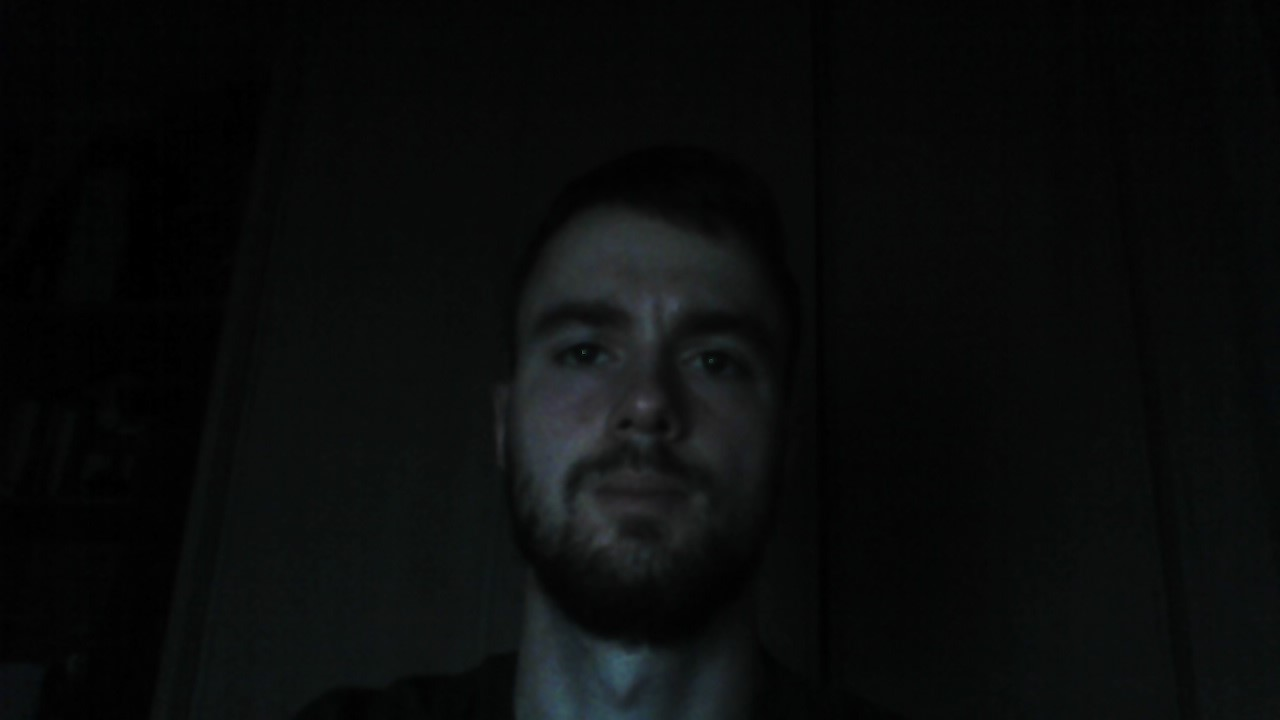
\includegraphics[width=\linewidth, height=20mm]{detekcja/11_input.jpg}
    	\end{minipage}
		& 
		\begin{minipage}{.2\textwidth}
      	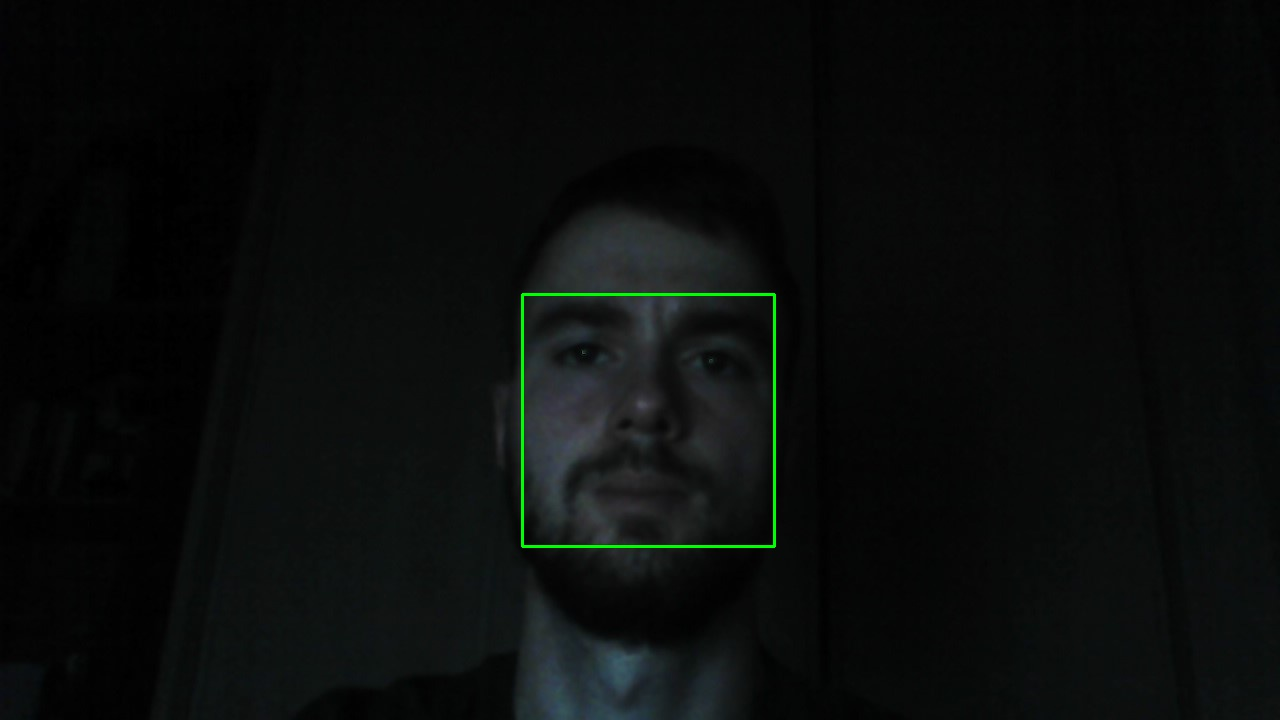
\includegraphics[width=\linewidth, height=20mm]{detekcja/11_haar.jpg}
    	\end{minipage}
		& 
		\begin{minipage}{.2\textwidth}
      	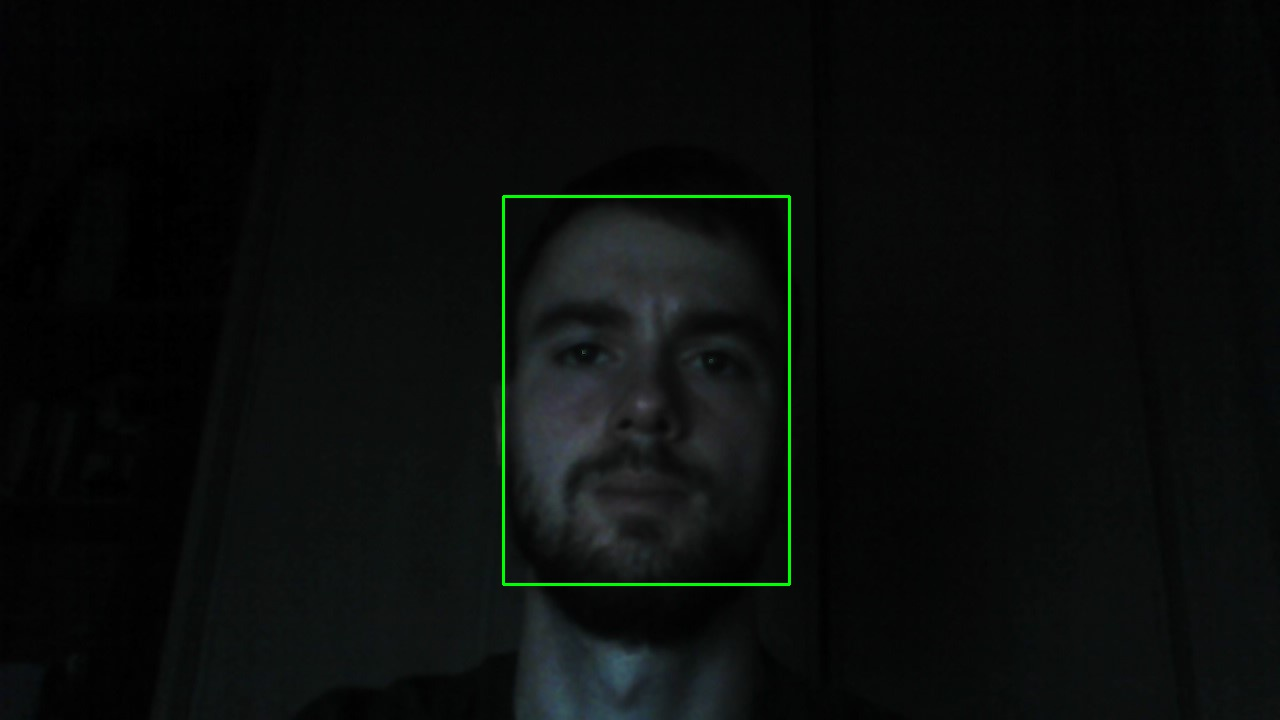
\includegraphics[width=\linewidth, height=20mm]{detekcja/11_dnn.jpg}
    	\end{minipage}
		& 
		\begin{minipage}{.2\textwidth}
      	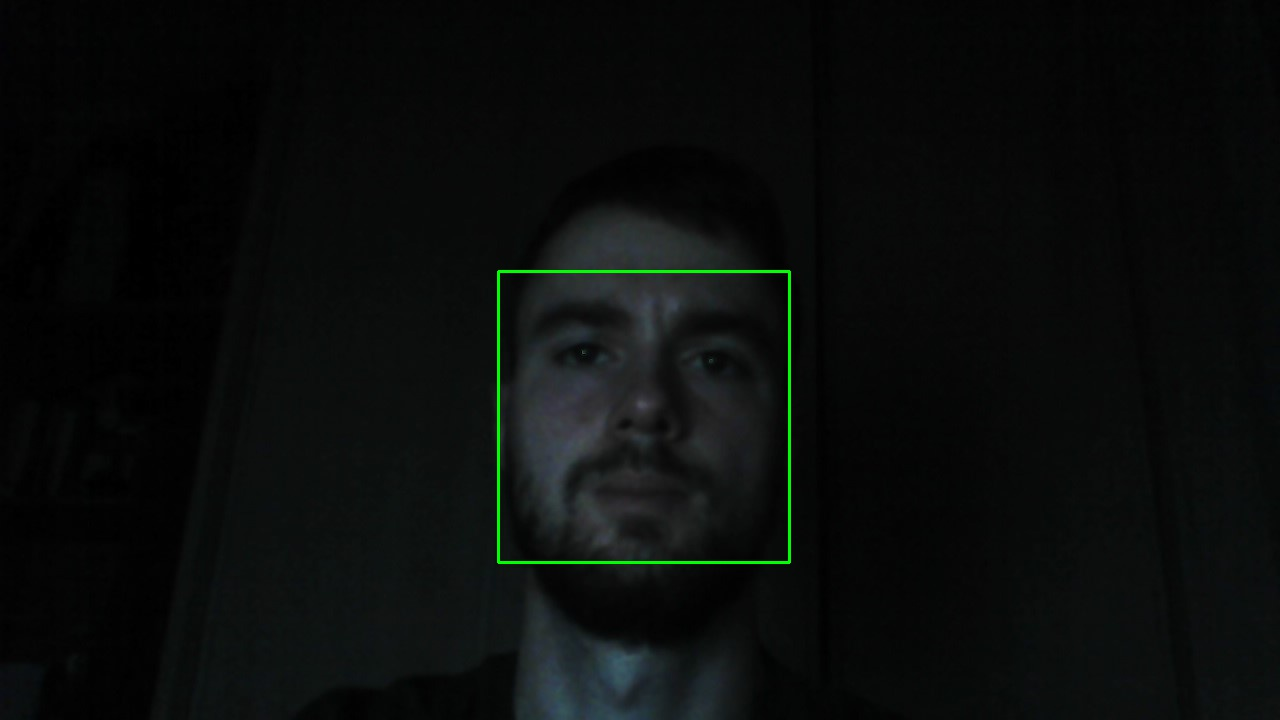
\includegraphics[width=\linewidth, height=20mm]{detekcja/11_azure.jpg}
    	\end{minipage}	
		\\
  		\hline
  		9&  		  		\begin{minipage}{.2\textwidth}
      	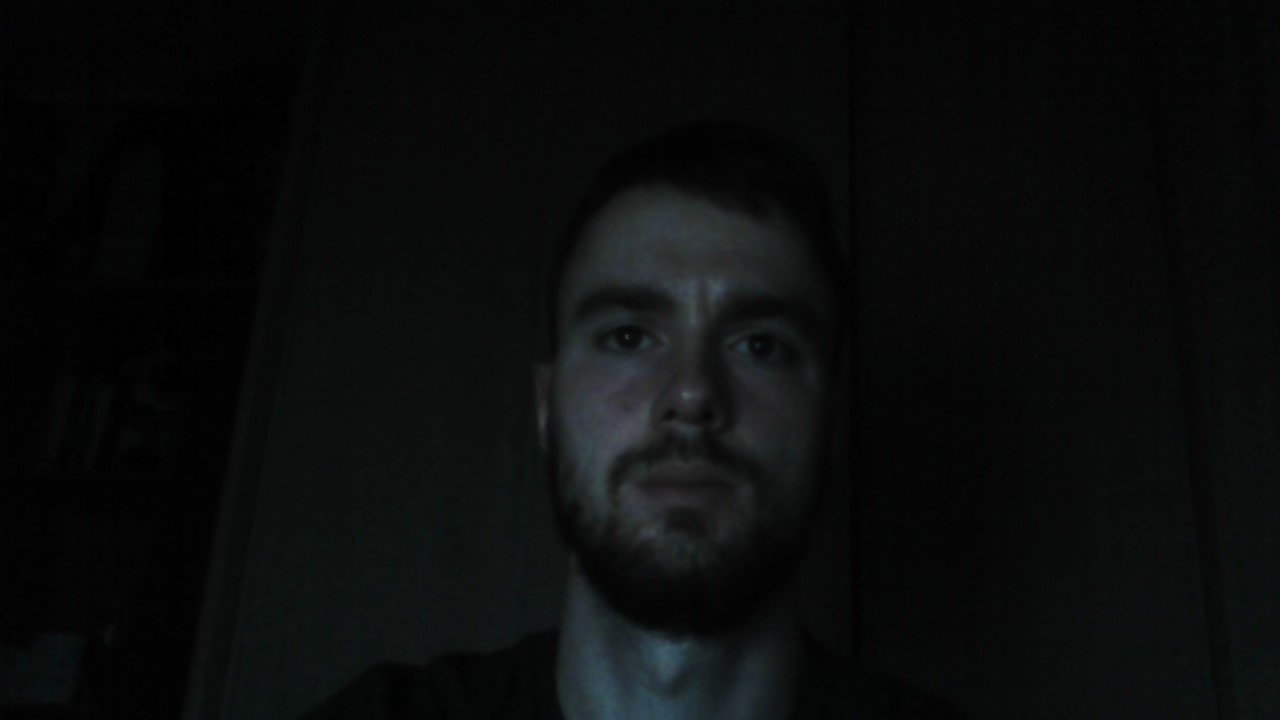
\includegraphics[width=\linewidth, height=20mm]{detekcja/12_input.jpg}
    	\end{minipage}
		& 
		\begin{minipage}{.2\textwidth}
      	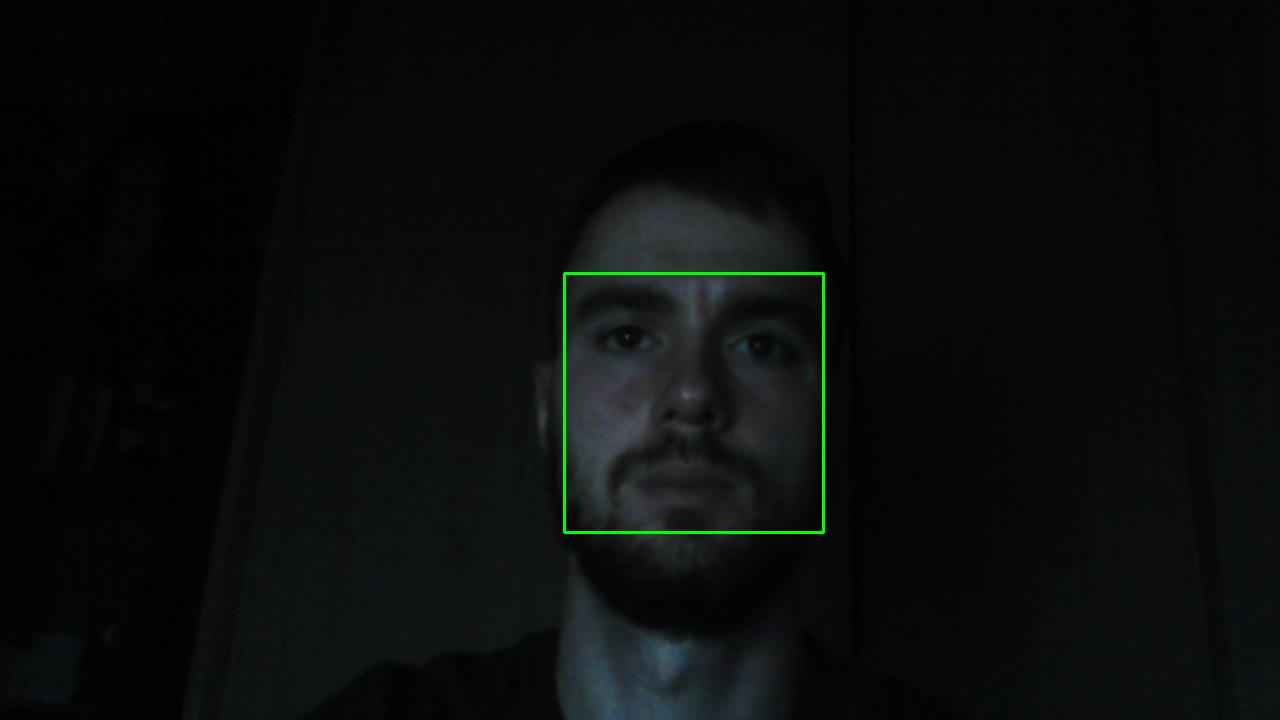
\includegraphics[width=\linewidth, height=20mm]{detekcja/12_haar.jpg}
    	\end{minipage}
		& 
		\begin{minipage}{.2\textwidth}
      	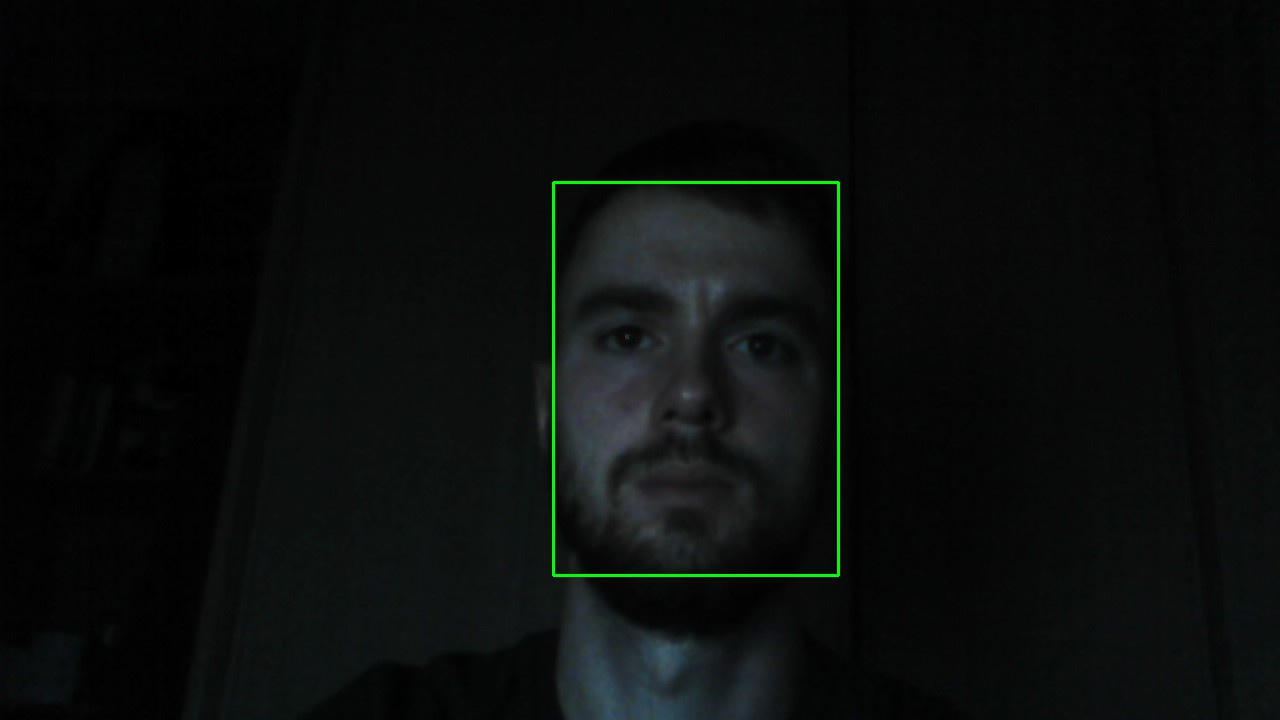
\includegraphics[width=\linewidth, height=20mm]{detekcja/12_dnn.jpg}
    	\end{minipage}
		& 
		\begin{minipage}{.2\textwidth}
      	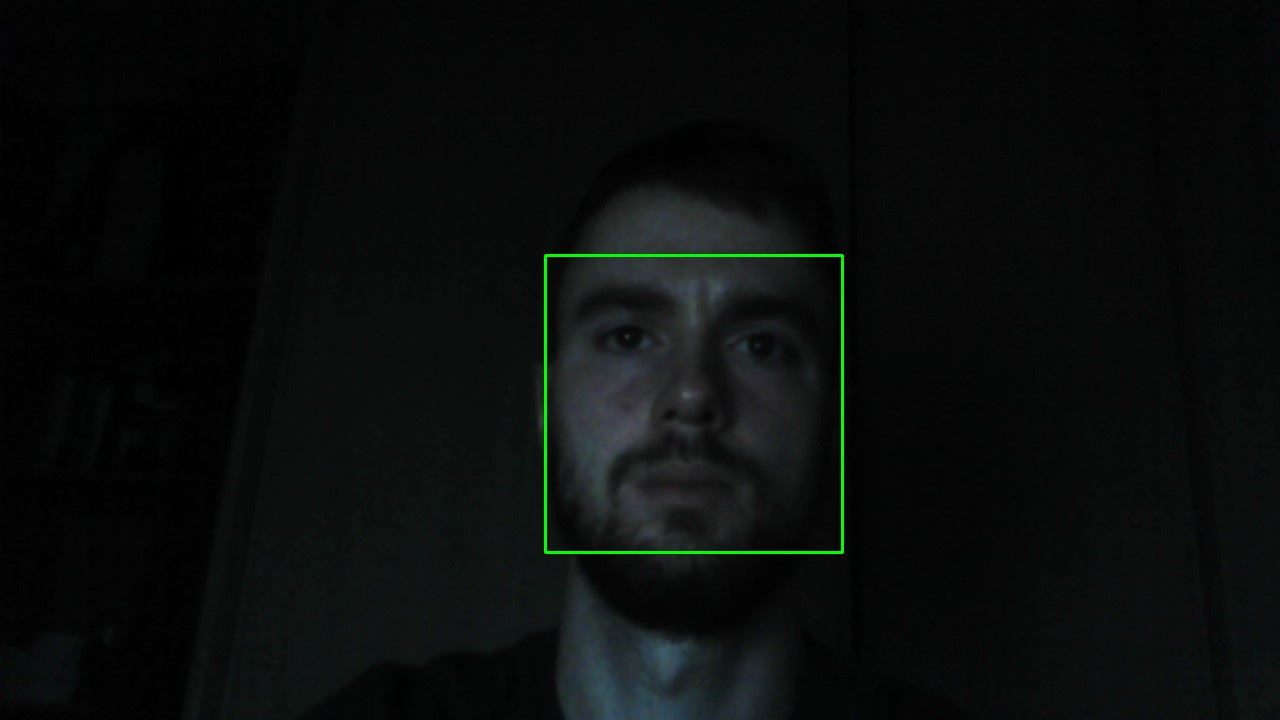
\includegraphics[width=\linewidth, height=20mm]{detekcja/12_azure.jpg}
    	\end{minipage}	
    	\\
  		\hline 
\caption{Porównanie działania detektorów w wybranych warunkach}
\label{tab:porownanie_detektorow}
\end{longtable}

\begin{table}[H]\label{tab:systemy}
	\centering
	\caption{Średni czas przetwarzania zadania detekcji twarzy}
	\scalebox{1.0}{
	\begin{tabular}{|c|c|c|c|}
  		\hline 
  		 & \bfseries Haar & \bfseries Dnn & \bfseries ACS\\
  		\hline
  		\bfseries Średni czas odpowiedzi [s]& 0,023127109 &0,018201053 &0,465438843 \\
  		\hline
  	\end{tabular}
  	}
\end{table}

\subsection{Wnioski}

\section{Dane treningowe}
Za dane wejściowe do procesu trenowania sieci neuronowych wybrano \fnurl{Glasgow Unfamiliar Face Database (GUFD)}{http://www.facevar.com/glasgow-unfamiliar-face-database}, która dostępna jest za darmo i można jej używać na potrzeby badań uczelnianych oraz publikacji. Jedynym warunkiem użycia jest zacytowanie jednej z publikacji właściciela bazy.

Baza zawiera 303 tożsamości. Na każdą z tożsamości składa się 20 zdjęć jednej osoby wykonanych w różnych warunkach np. różniące się kąty ujęcia, wyrazy twarzy oraz z dodatkowymi akcesoriami(okulary, kaptur, czapka). 

Do materiałów uczących dodatkowo dodano profil autora tej pracy magisterskiej.

\section{Trenowanie sieci neuronowych}
Podczas badania sieci neuronowych postanowiono sprawdzić kilka podstawowych czynników, na które składa się wpływ ilości wybranych tożsamości oraz wpływ ilości zdjęć przydzielonych tożsamości na:
\begin{itemize}
\item czas potrzebny na preprocessing danych uczących,
\item czas trwania trenowania modelu,
\item rozmiar pliku zawierającego model (jeśli istnieje).
\end{itemize}
W rozdziale \ref{b:rozpoznawanie} omówiono wpływ wyżej wymienionych parametrów na czas oraz pewność identyfikowania tożsamości.

\subsection{Wpływ wybranych parametrów na czas trwania przygotowania danych uczących}
\begin{figure}[H]
	\centering
	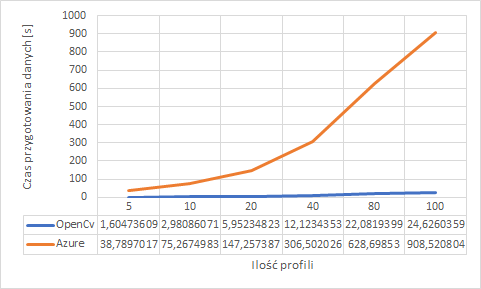
\includegraphics[scale=1.0]{czas_przygotowania_a_ilosc_profili.png}
	\caption{Wpływ ilości profili użytych podczas treningu na czas przygotowania danych uczących}
	\label{fig:czas_p_profile}
\end{figure}

\begin{figure}[H]
	\centering
	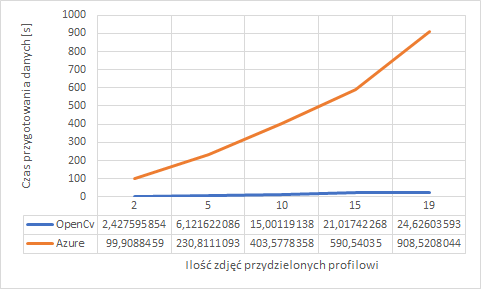
\includegraphics[scale=1.0]{czas_przygotowania_a_ilosc_zdjec.png}
	\caption{Wpływ ilości zdjęć przydzielonych profilowi na czas przygotowania danych uczących}
	\label{fig:czas_p_zdjecia}
\end{figure}

\subsection{Wpływ wybranych parametrów na czas trwania treningu}
\begin{figure}[H]
	\centering
	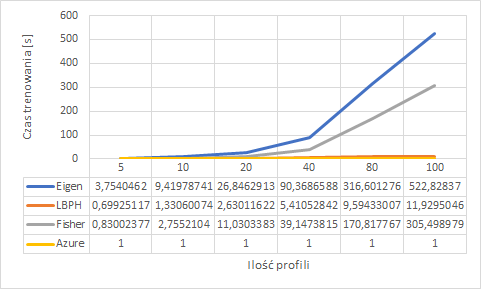
\includegraphics[scale=1.0]{czas_trenowania_a_ilosc_profili.png}
	\caption{Wpływ ilości profili użytych podczas treningu na czas trenowania sieci}
	\label{fig:czas_t_profile}
\end{figure}

\begin{figure}[H]
	\centering
	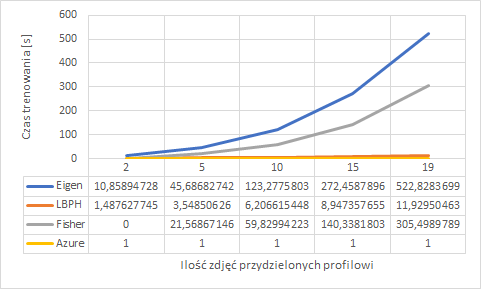
\includegraphics[scale=1.0]{czas_trenowania_a_ilosc_zdjec.png}
	\caption{Wpływ ilości zdjęć przydzielonych profilowi na czas trenowania sieci}
	\label{fig:czas_t_zdjecia}
\end{figure}

\subsection{Wpływ wybranych parametrów na rozmiar modelu sieci}
\begin{figure}[H]
	\centering
	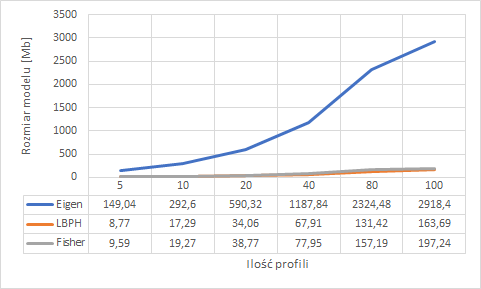
\includegraphics[scale=1.0]{rozmiar_modelu_a_ilosc_profili.png}
	\caption{Wpływ ilości profili użytych podczas treningu na rozmiar utworzonego modelu}
	\label{fig:rozmiar_profile}
\end{figure}

\begin{figure}[H]
	\centering
	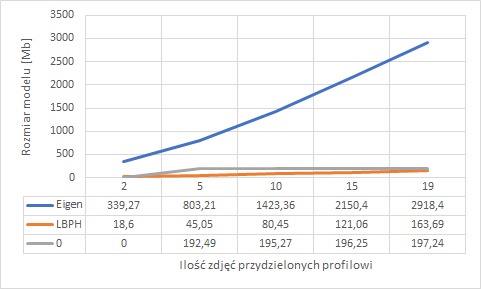
\includegraphics[scale=1.0]{rozmiar_modelu_a_ilosc_zdjec.png}
	\caption{Wpływ ilości zdjęć przydzielonych profilowi na rozmiar utworzonego modelu}
	\label{fig:rozmiar_zdjecia}
\end{figure}

\section{Rozpoznawanie twarzy} \label{b:rozpoznawanie}
\subsection{Wpływ ilości zdjęć przypisanych profilowi na pewność rozpoznania}
\begin{figure}[H]
	\centering
	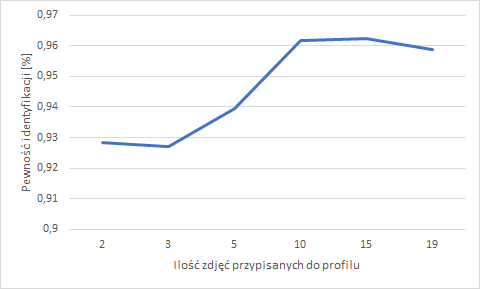
\includegraphics[scale=1.0]{azure_pewnosc_a_ilosc_zdjec.png}
	\caption{Wpływ ilości zdjęć przydzielonych profilowi na pewność identyfikacji Azure. Użyto 100 profili}
	\label{fig:azure_zdjecia}
\end{figure}
\begin{figure}[H]
	\centering
	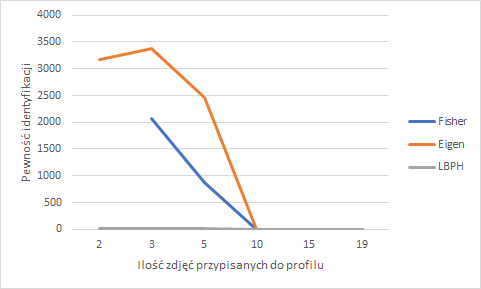
\includegraphics[scale=1.0]{opencv_pewnosc_a_ilosc_zdjec.png}
	\caption{Wpływ ilości zdjęć przydzielonych profilowi na pewność identyfikacji OpenCv. Użyto 100 profili}
	\label{fig:opencv_zdjecia}
\end{figure}

\subsection{Wpływ ilości profili użytych podczas treningu na pewność rozpoznania}
Przy 19 zdjeciach na profil, twarzy identyfikowane były bardzo dobrze i nie bylo widac roznicy w pewnosci identyfikacji.
\begin{figure}[H]
	\centering
	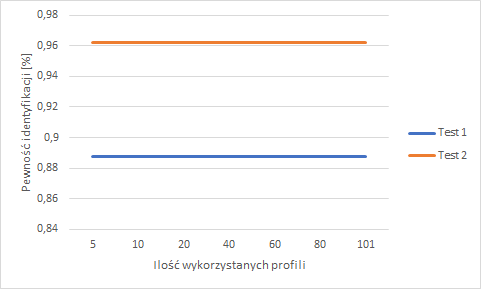
\includegraphics[scale=1.0]{10_azure_pewnosc_a_ilosc_profili.png}
	\caption{Wpływ ilości profili użytych podczas nauki na pewność identyfikacji Azure. Użyto 10 zdjęć dla każdego profilu}
	\label{fig:azure_10__profile}
\end{figure}
Przy 10 zdjęciach nie bylo roznicy dla metod OpenCv
\begin{figure}[H]
	\centering
	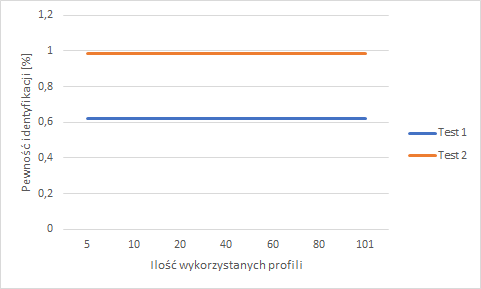
\includegraphics[scale=1.0]{5_azure_pewnosc_a_ilosc_profili.png}
	\caption{Wpływ ilości profili użytych podczas nauki na pewność identyfikacji Azure. Użyto 5 zdjęć dla każdego profilu}
	\label{fig:azure_5__profile}
\end{figure}
\begin{figure}[H]
	\centering
	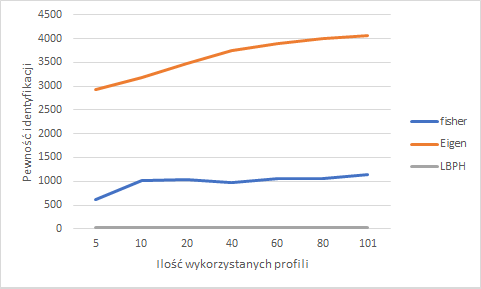
\includegraphics[scale=1.0]{5_opencv_pewnosc_a_ilosc_profili.png}
	\caption{Wpływ ilości profili użytych podczas nauki na pewność identyfikacji OpenCv. Użyto 5 zdjęć dla każdego profilu}
	\label{fig:azure_5__profile}
\end{figure}

\subsection{Porównanie wyników}
\subsection{Czas przetwarzania zapytania}

\section{Ocena przydatności wybranych usług IoT}



Konfiguracja bazy danych oraz maszyny wirtualnej okazała się równie prosta w każdym ze środowisk. Proces konfiguracji odbywał się poprzez wypełnienie kilku formularzy niewymagających wprowadzania dużej ilości informacji (ze względu na ograniczenia studenckiej licencji). Na końcu procesu uzyskany zostaje connection string oraz konto za pomocą, którego można zalogować się na serwer.

Największa różnica między dwoma dostawcami wystąpiła w przypadku usług hostujących aplikację webową czyli Azure App Service oraz AWS Elastic Beanstalk. Podczas pierwszych testów konfiguracji aplikacja internetowa istniała jedynie w rozwiązaniu przygotowanym w języku Angular 4. Struktura aplikacji została przygotowana na podstawie wzoru przygotowanego przez Microsoft. Azure App Service bezproblemowo wspierał nawet najnowsze wersje rozwiązań przygotowanych dla .NET Core 2. Niestety AWS nie był przygotowany 